\documentclass{article}
\usepackage{amsfonts}
\usepackage{amsmath}
\usepackage{fullpage}
% \usepackage{graphicx}
\usepackage[aux]{rerunfilecheck}
\usepackage{pgfplots}
\usepackage{tikz}
\usetikzlibrary{calc}
%\usepackage{pgfmath}

\newcommand{\ds}{\displaystyle}

% Macros for MATH 110 course dates

\newcommand{\commonTheme}{metropolis}
\newcommand{\commonColorTheme}{metropolis}

\newcommand{\commonAuthor}{Edward Doolittle}
\newcommand{\commonInstitute}{Department of Indigenous Knowledge and
  Science \\ First Nations University of Canada}
\newcommand{\commonCourse}{MATH 110 Calculus I}
\newcommand{\commonTerm}{202510}
\newcommand{\commonDate}{January 6, 2025}

% Review Material

% Lab 0
\newcommand{\commonEventNegativeOne}{LabNegativeOne}
\newcommand{\commonDateLabNegativeOne}{Monday, January 6, 2025}
\newcommand{\commonTitleLabNegativeOne}{MATH 110 Lab 0}
\newcommand{\commonSubtitleLabNegativeOne}{No Lab; Course Opens}

% Section 001
\newcommand{\commonEventZeroZeroOne}{ZeroZeroOne}
\newcommand{\commonDateZeroZeroOne}{Tuesday, January 7, 2025}
\newcommand{\commonTitleZeroZeroOne}{MATH 110 Review 0.1}
\newcommand{\commonSubtitleZeroZeroOne}{Review of Algebra}
\newcommand{\commonPSTitleZeroZeroOne}{MATH 110 Review Problem Set 0.1}

% Section 00A
\newcommand{\commonEventZeroZeroA}{ZeroZeroA}
\newcommand{\commonDateZeroZeroA}{Tuesday, January 7, 2025}
\newcommand{\commonTitleZeroZeroA}{MATH 110 Review 0.A}
\newcommand{\commonSubtitleZeroZeroA}{Review of Inequalities and
  Absolute Values}
\newcommand{\commonPSTitleZeroZeroA}{MATH 110 Review Problem Set 0.A}

% Section 00B
\newcommand{\commonEventZeroZeroB}{ZeroZeroB}
\newcommand{\commonDateZeroZeroB}{Tuesday, January 7, 2025}
\newcommand{\commonTitleZeroZeroB}{MATH 110 Review 0.B}
\newcommand{\commonSubtitleZeroZeroB}{Review of Coordinate Geometry
  and Lines}
\newcommand{\commonPSTitleZeroZeroB}{MATH 110 Review Problem Set 0.B}

% Section 00C
\newcommand{\commonEventZeroZeroC}{ZeroZeroC}
\newcommand{\commonDateZeroZeroC}{Thursday, January 9, 2025}
\newcommand{\commonTitleZeroZeroC}{MATH 110 Review 0.C}
\newcommand{\commonSubtitleZeroZeroC}{Review of Graphs of Second
  Degree Equations}
\newcommand{\commonPSTitleZeroZeroC}{MATH 110 Review Problem Set 0.C}

% Section 00D
\newcommand{\commonEventZeroZeroD}{ZeroZeroD}
\newcommand{\commonDateZeroZeroD}{Thursday, January 9, 2025}
\newcommand{\commonTitleZeroZeroD}{MATH 110 Review 0.D}
\newcommand{\commonSubtitleZeroZeroD}{Review of Trigonometry}
\newcommand{\commonPSTitleZeroZeroD}{MATH 110 Review Problem Set 0.D}

% Section 011
\newcommand{\commonEventZeroOneOne}{ZeroOneOne}
\newcommand{\commonDateZeroOneOne}{Thursday, January 9, 2025}
\newcommand{\commonTitleZeroOneOne}{MATH 110 Review 1.1}
\newcommand{\commonSubtitleZeroOneOne}{Review of Functions}
\newcommand{\commonPSTitleZeroOneOne}{MATH 110 Review Problem Set 1.1}


% Main Course

% Lab 1
\newcommand{\commonEventZero}{LabZero}
\newcommand{\commonDateLabZero}{Monday, January 13, 2025}
\newcommand{\commonTitleLabZero}{MATH 110 Lab 1}
\newcommand{\commonSubtitleLabZero}{Quiz 0: STACK, Onboarding}

% Section 1.4
\newcommand{\commonEventOne}{ZeroOneFour}
\newcommand{\commonDateZeroOneFour}{Tuesday, January 14, 2025}
\newcommand{\commonTitleZeroOneFour}{MATH 110 Lecture 1.4}
\newcommand{\commonSubtitleZeroOneFour}{The Tangent and Velocity Problems}
\newcommand{\commonPSTitleZeroOneFour}{MATH 110 Problem Set 1.4}

% Section 1.5
\newcommand{\commonEventTwo}{ZeroOneFive}
\newcommand{\commonDateZeroOneFive}{Thursday, January 16, 2025}
\newcommand{\commonTitleZeroOneFive}{MATH 110 Lecture 1.5}
\newcommand{\commonSubtitleZeroOneFive}{The Limit of a Function}
\newcommand{\commonPSTitleZeroOneFive}{MATH 110 Problem Set 1.5}

% Lab 2
\newcommand{\commonEventThree}{LabOne}
\newcommand{\commonDateLabOne}{Monday, January 20, 2025}
\newcommand{\commonTitleLabOne}{MATH 110 Lab 2}
\newcommand{\commonSubtitleLabOne}{Quiz 1: Review}

% Section 1.6
\newcommand{\commonEventFour}{ZeroOneSix}
\newcommand{\commonDateZeroOneSix}{Tuesday, January 21, 2025}
\newcommand{\commonTitleZeroOneSix}{MATH 110 Lecture 1.6}
\newcommand{\commonSubtitleZeroOneSix}{Calculating Limits Using the Limit Laws}
\newcommand{\commonPSTitleZeroOneSix}{MATH 110 Problem Set 1.6}

% Section 1.7
\newcommand{\commonEventFive}{ZeroOneSeven}
\newcommand{\commonDateZeroOneSeven}{(Not covered)}
\newcommand{\commonTitleZeroOneSeven}{MATH 110 Lecture 1.7}
\newcommand{\commonSubtitleZeroOneSeven}{The Precise Definition of a Limit}
\newcommand{\commonPSTitleZeroOneSeven}{MATH 110 Problem Set 1.7}

% Section 1.8
\newcommand{\commonEventSix}{ZeroOneEight}
\newcommand{\commonDateZeroOneEight}{Thursday, January 23, 2025}
\newcommand{\commonTitleZeroOneEight}{MATH 110 Lecture 1.8}
\newcommand{\commonSubtitleZeroOneEight}{Continuity}
\newcommand{\commonPSTitleZeroOneEight}{MATH 110 Problem Set 1.8}

% Lab 3
\newcommand{\commonEventSeven}{LabTwo}
\newcommand{\commonDateLabTwo}{Monday, January 27, 2025}
\newcommand{\commonTitleLabTwo}{MATH 110 Lab 3}
\newcommand{\commonSubtitleLabTwo}{Quiz 2: Sections 1.4, 1.5}

% Section 2.1
\newcommand{\commonEventEight}{ZeroTwoOne}
\newcommand{\commonDateZeroTwoOne}{Tuesday, January 28, 2025}
\newcommand{\commonTitleZeroTwoOne}{MATH 110 Lecture 2.1}
\newcommand{\commonSubtitleZeroTwoOne}{Derivatives and Rates of Change}
\newcommand{\commonPSTitleZeroTwoOne}{MATH 110 Problem Set 2.1}

% Section 2.2
\newcommand{\commonEventNine}{ZeroTwoTwo}
\newcommand{\commonDateZeroTwoTwo}{Thursday, January 30, 2025}
\newcommand{\commonTitleZeroTwoTwo}{MATH 110 Lecture 2.2}
\newcommand{\commonSubtitleZeroTwoTwo}{The Derivative as a Function}
\newcommand{\commonPSTitleZeroTwoTwo}{MATH 110 Problem Set 2.2}

% Lab 4
\newcommand{\commonEventTen}{LabThree}
\newcommand{\commonDateMTOne}{Monday, February 3, 2025} 
\newcommand{\commonDateLabThree}{Monday, February 3, 2025}
\newcommand{\commonTitleLabThree}{MATH 110 Lab 4}
\newcommand{\commonSubtitleLabThree}{Midterm: Review, Chapter 1}

% Section 2.3
\newcommand{\commonEventEleven}{ZeroTwoThree}
\newcommand{\commonDateZeroTwoThree}{Tuesday, February 4, 2025}
\newcommand{\commonTitleZeroTwoThree}{MATH 110 Lecture 2.3}
\newcommand{\commonSubtitleZeroTwoThree}{Differentiation Formulas}
\newcommand{\commonPSTitleZeroTwoThree}{MATH 110 Problem Set 2.3}

% Section 2.4
\newcommand{\commonEventTwelve}{ZeroTwoFour}
\newcommand{\commonDateZeroTwoFour}{Thursday, February 6, 2025}
\newcommand{\commonTitleZeroTwoFour}{MATH 110 Lecture 2.4}
\newcommand{\commonSubtitleZeroTwoFour}{Derivatives of Trigonometric Functions}
\newcommand{\commonPSTitleZeroTwoFour}{MATH 110 Problem Set 2.4}

% Lab 5
\newcommand{\commonEventThirteen}{LabFour}
\newcommand{\commonDateLabFour}{Monday, February 10, 2025}
\newcommand{\commonTitleLabFour}{MATH 110 Lab 5}
\newcommand{\commonSubtitleLabFour}{Quiz 3: Sections 2.1, 2.2}

% Section 2.5
\newcommand{\commonEventFourteen}{ZeroTwoFive}
\newcommand{\commonDateZeroTwoFive}{Tuesday, February 11, 2025}
\newcommand{\commonTitleZeroTwoFive}{MATH 110 Lecture 2.5}
\newcommand{\commonSubtitleZeroTwoFive}{The Chain Rule}
\newcommand{\commonPSTitleZeroTwoFive}{MATH 110 Problem Set 2.5}

% Section 2.6
\newcommand{\commonEventFifteen}{ZeroTwoSix}
\newcommand{\commonDateZeroTwoSix}{Thursday, February 13, 2025}
\newcommand{\commonTitleZeroTwoSix}{MATH 110 Lecture 2.6}
\newcommand{\commonSubtitleZeroTwoSix}{Implicit Differentiation}
\newcommand{\commonPSTitleZeroTwoSix}{MATH 110 Problem Set 2.6}

% Lab 6
\newcommand{\commonEventSixteen}{LabFive}
\newcommand{\commonDateLabFive}{Monday, February 24, 2025}
\newcommand{\commonTitleLabFive}{MATH 110 Lab 6}
\newcommand{\commonSubtitleLabFive}{Quiz 4: Sections 2.3, 2.4}

% Section 2.7
\newcommand{\commonEventSeventeen}{ZeroTwoSeven}
\newcommand{\commonDateZeroTwoSeven}{Tuesday, February 25, 2025}
\newcommand{\commonTitleZeroTwoSeven}{MATH 110 Lecture 2.7}
\newcommand{\commonSubtitleZeroTwoSeven}{Rates of Change in the
  Natural and Social Sciences}
\newcommand{\commonPSTitleZeroTwoSeven}{MATH 110 Problem Set 2.7}

% Section 2.8
\newcommand{\commonEventEighteen}{ZeroTwoEight}
\newcommand{\commonDateZeroTwoEight}{Thursday, February 27, 2025}
\newcommand{\commonTitleZeroTwoEight}{MATH 110 Lecture 2.8}
\newcommand{\commonSubtitleZeroTwoEight}{Related Rates}
\newcommand{\commonPSTitleZeroTwoEight}{MATH 110 Problem Set 2.8}

% Lab 7
\newcommand{\commonEventNineteen}{LabSix}
\newcommand{\commonDateLabSix}{Monday, March 3, 2025}
\newcommand{\commonTitleLabSix}{MATH 110 Lab 7}
\newcommand{\commonSubtitleLabSix}{Quiz 5: Sections 2.5, 2.6}

% Section 3.1
\newcommand{\commonEventTwenty}{ZeroThreeOne}
\newcommand{\commonDateZeroThreeOne}{Tuesday, March 4, 2025}
\newcommand{\commonTitleZeroThreeOne}{MATH 110 Lecture 3.1}
\newcommand{\commonSubtitleZeroThreeOne}{Maximum and Minimum Values}
\newcommand{\commonPSTitleZeroThreeOne}{MATH 11 Problem Set 3.1}

% Section 3.2
\newcommand{\commonEventTwentyOne}{ZeroThreeTwo}
\newcommand{\commonDateZeroThreeTwo}{Thursday, March 6, 2025}
\newcommand{\commonTitleZeroThreeTwo}{MATH 110 Lecture 3.2}
\newcommand{\commonSubtitleZeroThreeTwo}{The Mean Value Theorem}
\newcommand{\commonPSTitleZeroThreeTwo}{MATH 110 Problem Set 3.2}

% Lab 8
\newcommand{\commonEventTwentyTwo}{LabSeven}
\newcommand{\commonDateMTTwo}{Monday, March 10, 2025}
\newcommand{\commonDateLabSeven}{Monday, March 10, 2025}
\newcommand{\commonTitleLabSeven}{MATH 110 Lab 8}
\newcommand{\commonSubtitleLabSeven}{Midterm: Chapter 2}

% Section 3.3
\newcommand{\commonEventTwentyThree}{ZeroThreeThree}
\newcommand{\commonDateZeroThreeThree}{Tuesday, March 11, 2025}
\newcommand{\commonTitleZeroThreeThree}{MATH 110 Lecture 3.3}
\newcommand{\commonSubtitleZeroThreeThree}{How Derivatives Affect the
  Shape of a Graph}
\newcommand{\commonPSTitleZeroThreeThree}{MATH 110 Problem Set 3.3}

% Section 3.4
\newcommand{\commonEventTwentyFour}{ZeroThreeFour}
\newcommand{\commonDateZeroThreeFour}{Thursday, March 13, 2025}
\newcommand{\commonTitleZeroThreeFour}{MATH 110 Lecture 3.4}
\newcommand{\commonSubtitleZeroThreeFour}{Limits at Infinity;
  Horizontal Asymptotes}
\newcommand{\commonPSTitleZeroThreeFour}{MATH 110 Problem Set 3.4}

% Lab 9
\newcommand{\commonEventTwentyFive}{LabEight}
\newcommand{\commonDateLabEight}{Monday, March 17, 2025}
\newcommand{\commonTitleLabEight}{MATH 110 Lab 9}
\newcommand{\commonSubtitleLabEight}{Quiz 6: Sections 3.1, 3.2}

% Section 3.5
\newcommand{\commonEventTwentySix}{ZeroThreeFive}
\newcommand{\commonDateZeroThreeFive}{Tuesday, March 18, 2025}
\newcommand{\commonTitleZeroThreeFive}{MATH 110 Lecture 3.5}
\newcommand{\commonSubtitleZeroThreeFive}{Summary of Curve Sketching}
\newcommand{\commonPSTitleZeroThreeFive}{MATH 110 Problem Set 3.5}

% Section 3.7
\newcommand{\commonEventTwentySeven}{ZeroThreeSeven}
\newcommand{\commonDateZeroThreeSeven}{Thursday, March 20, 2025}
\newcommand{\commonTitleZeroThreeSeven}{MATH 110 Lecture 3.7}
\newcommand{\commonSubtitleZeroThreeSeven}{Optimization Problems}
\newcommand{\commonPSTitleZeroThreeSeven}{MATH 110 Problem Set 3.7}

% Lab 10
\newcommand{\commonEventTwentyEight}{LabNine}
\newcommand{\commonDateLabNine}{Monday, March 24, 2025}
\newcommand{\commonTitleLabNine}{MATH 110 Lab 10}
\newcommand{\commonSubtitleLabNine}{Quiz 7: Sections 3.3, 3.4}

% Section 4.1
\newcommand{\commonEventTwentyNine}{ZeroFourOne}
\newcommand{\commonDateZeroFourOne}{Tuesday, March 25, 2025}
\newcommand{\commonTitleZeroFourOne}{MATH 110 Lecture 4.1}
\newcommand{\commonSubtitleZeroFourOne}{Areas and Distances}
\newcommand{\commonPSTitleZeroFourOne}{MATH 110 Problem Set 4.1}

% Section 4.2
\newcommand{\commonEventThirty}{ZeroFourTwo}
\newcommand{\commonDateZeroFourTwo}{Thursday, March 27, 2025}
\newcommand{\commonTitleZeroFourTwo}{MATH 110 Lecture 4.2}
\newcommand{\commonSubtitleZeroFourTwo}{The Definite Integral}
\newcommand{\commonPSTitleZeroFourTwo}{MATH 110 Problem Set 4.2}

% Lab 11
\newcommand{\commonEventThirtyOne}{LabTen}
\newcommand{\commonDateLabTen}{Monday, March 31, 2025}
\newcommand{\commonTitleLabTen}{MATH 110 Lab 11}
\newcommand{\commonSubtitleLabTen}{Quiz 8: Sections 3.5, 3.7}

% Section 4.3
\newcommand{\commonEventThirtyTwo}{ZeroFourThree}
\newcommand{\commonDateZeroFourThree}{Tuesday, April 1, 2025}
\newcommand{\commonTitleZeroFourThree}{MATH 110 Lecture 4.3}
\newcommand{\commonSubtitleZeroFourThree}{The Fundamental Theorem of Calculus}
\newcommand{\commonPSTitleZeroFourThree}{MATH 110 Problem Set 4.3}

% Section 4.4
\newcommand{\commonEventThirtyThree}{ZeroFourFour}
\newcommand{\commonDateZeroFourFour}{Thursday, April 3, 2025}
\newcommand{\commonTitleZeroFourFour}{MATH 110 Lecture 4.4}
\newcommand{\commonSubtitleZeroFourFour}{Indefinite Integrals and the
  Net Change Theorem}
\newcommand{\commonPSTitleZeroFourFour}{MATH 110 Problem Set 4.4}

% Lab 12
\newcommand{\commonEventThirtyFour}{LabEleven}
\newcommand{\commonDateLabEleven}{Monday, April 7, 2025}
\newcommand{\commonTitleLabEleven}{MATH 110 Lab 12}
\newcommand{\commonSubtitleLabEleven}{Quiz 9: Sections 4.1, 4.2}

% Section 4.5
\newcommand{\commonEventThirtyFive}{ZeroFourFive}
\newcommand{\commonDateZeroFourFive}{Tuesday, April 8, 2025}
\newcommand{\commonTitleZeroFourFive}{MATH 110 Lecture 4.5}
\newcommand{\commonSubtitleZeroFourFive}{The Substitution Rule}
\newcommand{\commonPSTitleZeroFourFive}{MATH 110 Problem Set 4.5}

% Section 5.1
\newcommand{\commonEventThirtySix}{ZeroFiveOne}
\newcommand{\commonDateZeroFiveOne}{Thursday, April 10, 2025}
\newcommand{\commonTitleZeroFiveOne}{MATH 110 Lecture 5.1}
\newcommand{\commonSubtitleZeroFiveOne}{Areas Between Curves}
\newcommand{\commonPSTitleZeroFiveOne}{MATH 110 Problem Set 5.1}

% Lab 13
\newcommand{\commonEventThirtySeven}{LabTwelve}
\newcommand{\commonDateLabTwelve}{Monday, April 14, 2025}
\newcommand{\commonTitleLabTwelve}{MATH 110 Review Lab}
\newcommand{\commonSubtitleLabTwelve}{Bonus Quiz 10: Sections 4.3, 4.4}

% Final Class
\newcommand{\commonEventThirtyEight}{FinalClass}
\newcommand{\commonDateFinalClass}{Tuesday, April 15, 2025}
\newcommand{\commonTitleFinalClass}{MATH 110 Review Class}
\newcommand{\commonSubtitleFinalClass}{Answer Questions, Review for Exam}

% Final Exam
\newcommand{\commonEventThirtyNine}{Final}
\newcommand{\commonDateFinal}{Thursday, April 22, 2025}
\newcommand{\commonTitleFinal}{MATH 110 Final Exam}
\newcommand{\commonSubtitleFinal}{Comprehensive Exam: All Sections}

% Orphaned -- no longer part of the course

% Section 2.9
\newcommand{\commonDateZeroTwoNine}{Not part of the course}
\newcommand{\commonTitleZeroTwoNine}{MATH 110 Lecture 2.9}
\newcommand{\commonSubtitleZeroTwoNine}{Linear Approximations and Differentials}
\newcommand{\commonPSTitleZeroTwoNine}{MATH 110 Problem Set 2.9}


% % Introduction
% \newcommand{\commonEventOneDate}{Wednesday, September 8, 2010}
% \newcommand{\commonEventOneDesc}{Introduction to the Course}
% \newcommand{\commonDateZeroZeroZero}{September 8, 2010}
% \newcommand{\commonTitleZeroZeroZero}{MATH 104 Introduction}
% \newcommand{\commonSubtitleZeroZeroZero}{Outline of the Course}

% % Lecture 1
% \newcommand{\commonEventTwoDate}{Friday, September 10, 2010}
% \newcommand{\commonEventTwoDesc}{Lecture 1: Algebra}
% \newcommand{\commonDateZeroZeroOne}{September 10, 2010}
% \newcommand{\commonTitleZeroZeroOne}{MATH 104 Lecture 1}
% \newcommand{\commonSubtitleZeroZeroOne}{Review of Algebra}
% % associated evaluation ... factor this out?
% \newcommand{\commonPSTitleZeroZeroOne}{MATH 104 Problem Set 1}
% \newcommand{\commonEvalZeroZeroOne}{Quiz 1}
% \newcommand{\commonEvalDateZeroZeroOne}{Wednesday, September 15, 2010}

% % Lecture 2
% \newcommand{\commonEventThreeDate}{Monday, September 13, 2010}
% \newcommand{\commonEventThreeDesc}{Lecture 2: Appendix A}
% \newcommand{\commonDateZeroZeroA}{September 13, 2010}
% \newcommand{\commonTitleZeroZeroA}{MATH 104 Lecture 2}
% \newcommand{\commonSubtitleZeroZeroA}{Appendix A: Numbers, Inequalities, 
%   and Absolute Values}
% % associated evaluation ... factor this out?
% \newcommand{\commonPSTitleZeroZeroA}{MATH 104 Problem Set 2}
% \newcommand{\commonEvalZeroZeroA}{Quiz 2}
% \newcommand{\commonEvalDateZeroZeroA}{Wednesday, September 22, 2010}

% % Review 1
% \newcommand{\commonEventFourDate}{Wednesday, September 15, 2010}
% \newcommand{\commonEventFourDesc}{Review 1: Review Algebra; Quiz 1; Review Appendix A}
% \newcommand{\commonDateRZeroOne}{September 15, 2010}
% \newcommand{\commonTitleRZeroOne}{MATH 104 Review 1}
% \newcommand{\commonSubtitleRZeroOne}{Review of Algebra, Appendix A}

% % Lecture 3
% \newcommand{\commonEventFiveDate}{Friday, September 17, 2010}
% \newcommand{\commonEventFiveDesc}{Lecture 3: Appendix B}
% \newcommand{\commonDateZeroZeroB}{September 17, 2010}
% \newcommand{\commonTitleZeroZeroB}{MATH 104 Lecture 3}
% \newcommand{\commonSubtitleZeroZeroB}{Appendix B: Coordinate Geometry and Lines}
% % associated evaluation ... factor this out?
% \newcommand{\commonPSTitleZeroZeroB}{MATH 104 Problem Set 3}
% \newcommand{\commonEvalZeroZeroB}{Quiz 2}
% \newcommand{\commonEvalDateZeroZeroB}{Wednesday, September 22, 2010}

% % Lecture 4
% \newcommand{\commonEventSixDate}{Monday, Sepbember 20, 2010}
% \newcommand{\commonEventSixDesc}{Lecture 4: Appendix C}
% \newcommand{\commonDateZeroZeroC}{September 20, 2010}
% \newcommand{\commonTitleZeroZeroC}{MATH 104 Lecture 4}
% \newcommand{\commonSubtitleZeroZeroC}{Appendix C: Graphs of Second-Degree Equations}
% % associated evaluation ... factor this out?
% \newcommand{\commonPSTitleZeroZeroC}{MATH 104 Problem Set 4}
% \newcommand{\commonEvalZeroZeroC}{Midterm 0}
% \newcommand{\commonEvalDateZeroZeroC}{Wednesday, September 29, 2010}

% % Review 2
% \newcommand{\commonEventSevenDate}{Wednesday, September 22, 2010}
% \newcommand{\commonEventSevenDesc}{Review 2: Review Appendix B; Quiz 2; Review Appendix C}
% \newcommand{\commonDateRZeroTwo}{September 22, 2010}
% \newcommand{\commonTitleRZeroTwo}{MATH 104 Review 2}
% \newcommand{\commonSubtitleRZeroTwo}{Review of Appendices B and C}

% % Lecture 5
% \newcommand{\commonEventEightDate}{Friday, September 24, 2010}
% \newcommand{\commonEventEightDesc}{Lecture 5: Appendix D}
% \newcommand{\commonDateZeroZeroD}{September 24, 2010}
% \newcommand{\commonTitleZeroZeroD}{MATH 104 Lecture 5}
% \newcommand{\commonSubtitleZeroZeroD}{Appendix D: Trigonometry}
% % associated evaluation ... factor this out?
% \newcommand{\commonPSTitleZeroZeroD}{MATH 104 Problem Set 5}
% \newcommand{\commonEvalZeroZeroD}{Midterm 0}
% \newcommand{\commonEvalDateZeroZeroD}{Wednesday, September 29, 2010}

% % Lecture 6
% \newcommand{\commonEventNineDate}{Monday, September 27, 2010}
% \newcommand{\commonEventNineDesc}{Lecture 6: Section 1.1}
% \newcommand{\commonDateZeroOneOne}{September 27, 2010}
% \newcommand{\commonTitleZeroOneOne}{MATH 104 Lecture 6}
% \newcommand{\commonSubtitleZeroOneOne}{Section 1.1: Four Ways to Represent a Function}
% % associated evaluation ... factor this out?
% \newcommand{\commonPSTitleZeroOneOne}{MATH 104 Problem Set 6}
% \newcommand{\commonEvalZeroOneOne}{Quiz 3}
% \newcommand{\commonEvalDateZeroOneOne}{Wednesday, October 6, 2010}

% % Review 3
% \newcommand{\commonEventTenDate}{Wednesday, September 29, 2010}
% \newcommand{\commonEventTenDesc}{Review 3: Review Appendix D; 
%   Self-Assessment Midterm 0}
% \newcommand{\commonDateRZeroThree}{September 29, 2010}
% \newcommand{\commonTitleRZeroThree}{MATH 104 Review 3}
% \newcommand{\commonSubtitleRZeroThree}{Review of Appendix D}

% % Lecture 7
% \newcommand{\commonEventElevenDate}{Friday, October 1, 2010}
% \newcommand{\commonEventElevenDesc}{Lecture 7: Section 1.2}
% \newcommand{\commonDateZeroOneTwo}{October 1, 2010}
% \newcommand{\commonTitleZeroOneTwo}{MATH 104 Lecture 7}
% \newcommand{\commonSubtitleZeroOneTwo}{Section 1.2: Mathematical Models: A Catalog of Essential Functions}
% % associated evaluation ... factor this out?
% \newcommand{\commonPSTitleZeroOneTwo}{MATH 104 Problem Set 7}
% \newcommand{\commonEvalZeroOneTwo}{Quiz 3}
% \newcommand{\commonEvalDateZeroOneTwo}{Wednesday, October 6, 2010}

% % Lecture 8
% \newcommand{\commonEventTwelveDate}{Monday, October 4, 2010}
% \newcommand{\commonEventTwelveDesc}{Lecture 8: Section 1.3}
% \newcommand{\commonDateZeroOneThree}{October 4, 2010}
% \newcommand{\commonTitleZeroOneThree}{MATH 104 Lecture 8}
% \newcommand{\commonSubtitleZeroOneThree}{Section 1.3: New Functions from Old Functions}
% % associated evaluation ... factor this out?
% \newcommand{\commonPSTitleZeroOneThree}{MATH 104 Problem Set 8}
% \newcommand{\commonEvalZeroOneThree}{Quiz 4}
% \newcommand{\commonEvalDateZeroOneThree}{Wednesday, October 13, 2010}

% % Review 4
% \newcommand{\commonEventThirteenDate}{Wednesday, October 6, 2010}
% \newcommand{\commonEventThirteenDesc}{Review 4: Review 1.1, 1.2; Quiz 3}
% \newcommand{\commonDateROneOne}{October 6, 2010}
% \newcommand{\commonTitleROneOne}{MATH 104 Review 4}
% \newcommand{\commonSubtitleROneOne}{Reveiw of 1.1, 1.2}

% % Lecture 9
% \newcommand{\commonEventFourteenDate}{Friday, October 8, 2010}
% \newcommand{\commonEventFourteenDesc}{Lecture 9: Section 1.4}
% \newcommand{\commonDateZeroOneFour}{October 8, 2010}
% \newcommand{\commonTitleZeroOneFour}{MATH 104 Lecture 9}
% \newcommand{\commonSubtitleZeroOneFour}{Section 1.4: Graphing Calculators and Computers}
% % associated evaluation ... factor this out?
% \newcommand{\commonPSTitleZeroOneFour}{MATH 104 Problem Set 9}
% \newcommand{\commonEvalZeroOneFour}{Quiz 4}
% \newcommand{\commonEvalDateZeroOneFour}{Wednesday, October 13, 2010}

% % Thanksgiving holiday
% \newcommand{\commonEventFifteenDate}{Monday, October 11, 2010}
% \newcommand{\commonEventFifteenDesc}{No class: Thanksgiving holiday}

% % Review 5
% \newcommand{\commonEventSixteenDate}{Wednesday, October 13, 2010}
% \newcommand{\commonEventSixteenDesc}{Review 5: Review 1.3, 1.4; Quiz 4}
% \newcommand{\commonDateROneTwo}{October 13, 2010}
% \newcommand{\commonTitleROneTwo}{MATH 104 Review 5}
% \newcommand{\commonSubtitleOneRTwo}{Review of 1.3, 1.4}

% % Lecture 10
% \newcommand{\commonEventSeventeenDate}{Friday, October 15, 2010}
% \newcommand{\commonEventSeventeenDesc}{Lecture 10: Section 1.5}
% \newcommand{\commonDateZeroOneFive}{October 15, 2010}
% \newcommand{\commonTitleZeroOneFive}{MATH 104 Lecture 10}
% \newcommand{\commonSubtitleZeroOneFive}{Section 1.5: Exponential Functions}
% % associated evaluation ... factor this out?
% \newcommand{\commonPSTitleZeroOneFive}{MATH 104 Problem Set 10}
% \newcommand{\commonEvalZeroOneFive}{Quiz 5}
% \newcommand{\commonEvalDateZeroOneFive}{Wednesday, October 20, 2010}

% % Lecture 11
% \newcommand{\commonEventEighteenDate}{Monday, October 18, 2010}
% \newcommand{\commonEventEighteenDesc}{Lecture 11: Section 1.6}
% \newcommand{\commonDateZeroOneSix}{October 18, 2010}
% \newcommand{\commonTitleZeroOneSix}{MATH 104 Lecture 11}
% \newcommand{\commonSubtitleZeroOneSix}{Section 1.6: Inverse Functions and Logarithms}
% % associated evaluation ... factor this out?
% \newcommand{\commonPSTitleZeroOneSix}{MATH 104 Problem Set 11}
% \newcommand{\commonEvalZeroOneSix}{Midterm 1}
% \newcommand{\commonEvalDateZeroOneSix}{Wednesday, October 27, 2010}

% % Review 6
% \newcommand{\commonEventNineteenDate}{Wednesday, October 20, 2010}
% \newcommand{\commonEventNineteenDesc}{Review 6: Review 1.5; Quiz 5; Review 1.6}
% \newcommand{\commonDateROneThree}{October 20, 2010}
% \newcommand{\commonDateZeroOneR}{October 20, 2010}
% \newcommand{\commonTitleROneThree}{MATH 104 Review 6}
% \newcommand{\commonSubtitleROneThree}{Review of 1.5, 1.6}
% % associated evaluation ... factor this out?
% \newcommand{\commonPSTitleZeroOneR}{MATH 104 Problem Set R1}
% \newcommand{\commonEvalZeroOneR}{Midterm 1}
% \newcommand{\commonEvalDateZeroOneR}{Wednesday, October 27, 2010}

% % Lecture 12
% \newcommand{\commonEventTwentyDate}{Friday, October 22, 2010}
% \newcommand{\commonEventTwentyDesc}{Lecture 12: Section 2.1}
% \newcommand{\commonDateZeroTwoOne}{October 22, 2010}
% \newcommand{\commonTitleZeroTwoOne}{MATH 104 Lecture 12}
% \newcommand{\commonSubtitleZeroTwoOne}{Section 2.1: The Tangent and Velocity Problems}
% % associated evaluation ... factor this out?
% \newcommand{\commonPSTitleZeroTwoOne}{MATH 104 Problem Set 12}
% \newcommand{\commonEvalZeroTwoOne}{Quiz 6}
% \newcommand{\commonEvalDateZeroTwoOne}{Wednesday, November 3, 2010}

% % Lecture 13
% \newcommand{\commonEventTwentyOneDate}{Monday, October 25, 2010}
% \newcommand{\commonEventTwentyOneDesc}{Lecture 13: Section 2.2(a)}
% \newcommand{\commonDateZeroTwoTwoa}{October 25, 2010}
% \newcommand{\commonTitleZeroTwoTwoa}{MATH 104 Lecture 13}
% \newcommand{\commonSubtitleZeroTwoTwoa}{Section 2.2(a): The Limit of a Function I}
% % associated evaluation ... factor this out?
% \newcommand{\commonPSTitleZeroTwoTwoa}{MATH 104 Problem Set 13}
% \newcommand{\commonEvalZeroTwoTwoa}{Quiz 6}
% \newcommand{\commonEvalDateZeroTwoTwoa}{Wednesday, November 3, 2010}

% % Midterm Test 1
% % October 27, 2010
% \newcommand{\commonEventTwentyTwoDate}{Wednesday, October 27, 2010}
% \newcommand{\commonEventTwentyTwoDesc}{Midterm Test 1: Chapter 1}

% % Lecture 14
% \newcommand{\commonEventTwentyThreeDate}{Friday, October 29, 2010}
% \newcommand{\commonEventTwentyThreeDesc}{Lecture 14: Section 2.2(b)}
% \newcommand{\commonDateZeroTwoTwob}{October 29, 2010}
% \newcommand{\commonTitleZeroTwoTwob}{MATH 104 Lecture 14}
% \newcommand{\commonSubtitleZeroTwoTwob}{Section 2.2(b): The Limit of a Function II}
% % associated evaluation ... factor this out?
% \newcommand{\commonPSTitleZeroTwoTwob}{MATH 104 Problem Set 14}
% \newcommand{\commonEvalZeroTwoTwob}{Quiz 6}
% \newcommand{\commonEvalDateZeroTwoTwob}{Wednesday, November 3, 2010}

% % Lecture 15
% \newcommand{\commonEventTwentyFourDate}{Monday, November 1, 2010}
% \newcommand{\commonEventTwentyFourDesc}{Lecture 15: Section 2.3}
% \newcommand{\commonDateZeroTwoThree}{November 1, 2010}
% \newcommand{\commonTitleZeroTwoThree}{MATH 104 Lecture 15}
% \newcommand{\commonSubtitleZeroTwoThree}{Section 2.3: Calculating Limits Using the Limit Laws}
% % associated evaluation ... factor this out?
% \newcommand{\commonPSTitleZeroTwoThree}{MATH 104 Problem Set 15}
% \newcommand{\commonEvalZeroTwoThree}{Quiz 7}
% \newcommand{\commonEvalDateZeroTwoThree}{Wednesday, November 10, 2010}

% % Review 7
% \newcommand{\commonEventTwentyFiveDate}{Wednesday, November 3, 2010}
% \newcommand{\commonEventTwentyFiveDesc}{Review 7: Review 2.1, 2.2; Quiz 6; Review 2.3}
% \newcommand{\commonDateRTwoOne}{November 3, 2010}
% \newcommand{\commonTitleRTwoOne}{MATH 104 Review 7}
% \newcommand{\commonSubtitleRTwoOne}{Review of 2.1, 2.2, 2.3}

% % Lecture 16
% \newcommand{\commonEventTwentySixDate}{Friday, November 5, 2010}
% \newcommand{\commonEventTwentySixDesc}{Lecture 16: Section 2.5}
% \newcommand{\commonDateZeroTwoFive}{November 5, 2010}
% \newcommand{\commonTitleZeroTwoFive}{MATH 104 Lecture 16}
% \newcommand{\commonSubtitleZeroTwoFive}{Section 2.5: Continuity}
% % associated evaluation ... factor this out?
% \newcommand{\commonPSTitleZeroTwoFive}{MATH 104 Problem Set 16}
% \newcommand{\commonEvalZeroTwoFive}{Quiz 7}
% \newcommand{\commonEvalDateZeroTwoFive}{Wednesday, November 10, 2010}

% % Lecture 17
% \newcommand{\commonEventTwentySevenDate}{Monday, November 8, 2010}
% \newcommand{\commonEventTwentySevenDesc}{Lecture 17: Section 2.6}
% \newcommand{\commonDateZeroTwoSix}{November 8, 2010}
% \newcommand{\commonTitleZeroTwoSix}{MATH 104 Lecture 17}
% \newcommand{\commonSubtitleZeroTwoSix}{Section 2.6: Limits at Infinity: Horizontal Asymptotes}
% % associated evaluation ... factor this out?
% \newcommand{\commonPSTitleZeroTwoSix}{MATH 104 Problem Set 17}
% \newcommand{\commonEvalZeroTwoSix}{Quiz 8}
% \newcommand{\commonEvalDateZeroTwoSix}{Wednesday, November 17, 2010}

% % Review 8
% \newcommand{\commonEventTwentyEightDate}{Wednesday, November 10, 2010}
% \newcommand{\commonEventTwentyEightDesc}{Review 8: Review 2.5; Quiz 7; Review 2.6}
% \newcommand{\commonDateRTwoTwo}{November 10, 2010}
% \newcommand{\commonTitleRTwoTwo}{MATH 104 Review 8}
% \newcommand{\commonSubtitleRTwoTwo}{Review of 2.5, 2.6}

% % Lecture 18
% \newcommand{\commonEventTwentyNineDate}{Friday, November 12, 2010}
% \newcommand{\commonEventTwentyNineDesc}{Lecture 18: Section 2.7}
% \newcommand{\commonDateZeroTwoSeven}{November 12, 2010}
% \newcommand{\commonTitleZeroTwoSeven}{MATH 104 Lecture 18}
% \newcommand{\commonSubtitleZeroTwoSeven}{Section 2.7: Derivatives and Rates of Change}
% % associated evaluation ... factor this out?
% \newcommand{\commonPSTitleZeroTwoSeven}{MATH 104 Problem Set 18}
% \newcommand{\commonEvalZeroTwoSeven}{Quiz 8}
% \newcommand{\commonEvalDateZeroTwoSeven}{Wednesday, November 17, 2010}

% % Lecture 19
% \newcommand{\commonEventThirtyDate}{Monday, November 15, 2010}
% \newcommand{\commonEventThirtyDesc}{Lecture 19: Section 2.8}
% \newcommand{\commonDateZeroTwoEight}{November 15, 2010}
% \newcommand{\commonTitleZeroTwoEight}{MATH 104 Lecture 19}
% \newcommand{\commonSubtitleZeroTwoEight}{Section 2.8: The Derivative as a Function}
% % associated evaluation ... factor this out?
% \newcommand{\commonPSTitleZeroTwoEight}{MATH 104 Problem Set 19}
% \newcommand{\commonEvalZeroTwoEight}{Midterm 2}
% \newcommand{\commonEvalDateZeroTwoEight}{Wednesday, November 24, 2010}

% % Review 9
% % November 17, 2010
% \newcommand{\commonEventThirtyOneDate}{Wednesday, November 17, 2010}
% \newcommand{\commonEventThirtyOneDesc}{Review 9: Review 2.7; Quiz 8; Review 2.8}
% \newcommand{\commonDateRTwoThree}{November 17, 2010}
% \newcommand{\commonTitleRTwoThree}{MATH 104 Review 9}
% \newcommand{\commonSubtitleRTwoThree}{Review of 2.7, 2.8}

% % Lecture 20
% \newcommand{\commonEventThirtyTwoDate}{Friday, November 19, 2010}
% \newcommand{\commonEventThirtyTwoDesc}{Lecture 20: Section 3.1}
% \newcommand{\commonDateZeroThreeOne}{November 19, 2010}
% \newcommand{\commonTitleZeroThreeOne}{MATH 104 Lecture 20}
% \newcommand{\commonSubtitleZeroThreeOne}{Section 3.1: Derivatives of Polynomials and Exponential Functions}
% % associated evaluation ... factor this out?
% \newcommand{\commonPSTitleZeroThreeOne}{MATH 104 Problem Set 20}
% \newcommand{\commonEvalZeroThreeOne}{Quiz 9}
% \newcommand{\commonEvalDateZeroThreeOne}{Wednesday, December 1, 2010}

% % Lecture 21
% \newcommand{\commonEventThirtyThreeDate}{Monday, November 22, 2010}
% \newcommand{\commonEventThirtyThreeDesc}{Lecture 21: Section 3.2}
% \newcommand{\commonDateZeroThreeTwo}{November 22, 2010}
% \newcommand{\commonTitleZeroThreeTwo}{MATH 104 Lecture 21}
% \newcommand{\commonSubtitleZeroThreeTwo}{Section 3.2: The Product and Quotient Rules}
% % associated evaluation ... factor this out?
% \newcommand{\commonPSTitleZeroThreeTwo}{MATH 104 Problem Set 21}
% \newcommand{\commonEvalZeroThreeTwo}{Quiz 9}
% \newcommand{\commonEvalDateZeroThreeTwo}{Wednesday, December 1, 2010}

% % Midterm Test 2
% \newcommand{\commonEventThirtyFourDate}{Wednesday, November 24, 2010}
% \newcommand{\commonEventThirtyFourDesc}{Midterm Test 2: Chapter 2}

% % Lecture 22
% \newcommand{\commonEventThirtyFiveDate}{Friday, November 26, 2010}
% \newcommand{\commonEventThirtyFiveDesc}{Lecture 22: Section 3.3}
% \newcommand{\commonDateZeroThreeThree}{November 26, 2010}
% \newcommand{\commonTitleZeroThreeThree}{MATH 104 Lecture 22}
% \newcommand{\commonSubtitleZeroThreeThree}{Section 3.3: Derivatives of Trigonometric Functions}
% % associated evaluation ... factor this out?
% \newcommand{\commonPSTitleZeroThreeThree}{MATH 104 Problem Set 22}
% \newcommand{\commonEvalZeroThreeThree}{Quiz 9}
% \newcommand{\commonEvalDateZeroThreeThree}{Wednesday, December 1, 2010}

% % Lecture 23
% \newcommand{\commonEventThirtySixDate}{Monday, November 29, 2010}
% \newcommand{\commonEventThirtySixDesc}{Lecture 23: Section 3.4}
% \newcommand{\commonDateZeroThreeFour}{November 29, 2010}
% \newcommand{\commonTitleZeroThreeFour}{MATH 104 Lecture 23}
% \newcommand{\commonSubtitleZeroThreeFour}{Section 3.4: The Chain Rule}
% % associated evaluation ... factor this out?
% \newcommand{\commonPSTitleZeroThreeFour}{MATH 104 Problem Set 23}
% \newcommand{\commonEvalZeroThreeFour}{the final exam}
% \newcommand{\commonEvalDateZeroThreeFour}{Monday, December 13, 2010}

% % Review 10
% \newcommand{\commonEventThirtySevenDate}{Wednesday, December 1, 2010}
% \newcommand{\commonEventThirtySevenDesc}{Review 10: Review 3.1, 3.2, 3.3; Quiz 9}
% \newcommand{\commonDateRThreeTwo}{December 1, 2010}
% \newcommand{\commonTitleRThreeTwo}{MATH 104 Review 10}
% \newcommand{\commonSubtitleRThreeTwo}{Review of 3.1, 3.2, 3.3}

% % Lecture 24
% \newcommand{\commonEventThirtyEightDate}{Friday, December 3, 2010}
% \newcommand{\commonEventThirtyEightDesc}{Lecture 24: Section 3.5}
% \newcommand{\commonDateZeroThreeFive}{December 3, 2010}
% \newcommand{\commonTitleZeroThreeFive}{MATH 104 Lecture 24}
% \newcommand{\commonSubtitleZeroThreeFive}{Section 3.5: Implicit Differentiation}
% % associated evaluation ... factor this out?
% \newcommand{\commonPSTitleZeroThreeFive}{MATH 104 Problem Set 24}
% \newcommand{\commonEvalZeroThreeFive}{the final exam}
% \newcommand{\commonEvalDateZeroThreeFive}{Monday, December 13, 2010}

% % Lecture 25
% \newcommand{\commonEventThirtyNineDate}{Monday, December 6, 2010}
% \newcommand{\commonEventThirtyNineDesc}{Lecture 25: Section 3.6}
% \newcommand{\commonDateZeroThreeSix}{December 6, 2010}
% \newcommand{\commonTitleZeroThreeSix}{MATH 104 Lecture 25}
% \newcommand{\commonSubtitleZeroThreeSix}{Section 3.6: Derivatives of Logarithmic Functions}
% % associated evaluation ... factor this out?
% \newcommand{\commonPSTitleZeroThreeSix}{MATH 104 Problem Set 25}
% \newcommand{\commonEvalZeroThreeSix}{the final exam}
% \newcommand{\commonEvalDateZeroThreeSix}{Monday, December 13, 2010}

% % Review 11
% \newcommand{\commonEventFortyDate}{Wednesday, December 8, 2010}
% \newcommand{\commonEventFortyDesc}{(Bonus) Review 11: Review 3.4, 3.5, 3.6}
% \newcommand{\commonDateRThreeThree}{December 8, 2010}
% \newcommand{\commonTitleRThreeThree}{MATH 104 (Bonus) Review 11}
% \newcommand{\commonSubtitleRThreeThree}{Review of 3.4, 3.5, 3.6}

% % Final Exam
% % December 13, 2010
% \newcommand{\commonEventFinalDate}{Monday, December 13, 2010}
% \newcommand{\commonEventFinalDesc}{MATH 104 Final Exam}

%%% Local variables:
%%% mode: latex
%%% TeX-master: "MATH110-Syllabus.tex"
%%% End:

\title{\commonPSTitleZeroThreeFive\ Solutions}
\author{\commonAuthor}
\date{\commonDateZeroThreeFive}

\allowdisplaybreaks

% EJD: labels for special points on graphs
% EJD: combine pairs of graphs
\begin{document}
\maketitle
\begin{enumerate}
\item %1
  \begin{enumerate}
  \item %1a
    \begin{itemize}
    \item[A] Domain: a polynomial has domain all of $\mathbb{R}$.
    \item[B] Intercepts: $x=0$ implies $y=0^4-4(0)^2+4=4$, so $(0,4)$
      is the $y$-intercept.  $y=0$ implies $x^4-4x^2+4=0$.  Factoring,
      $(x^2-2)^2=0$ which implies $x^2-2=0$ so $x=\pm\sqrt{2}$.  The
      $x$-intercepts are $(-\sqrt{2},0)$ and $(\sqrt{2},0)$.
    \item[C] Symmetry: Since the function only contains even powers of
      $x$, it follows that $y(x)=y(-x)$, in other words the function
      is even, with mirror symmetry in the $y$-axis.
    \item[D] Asymptotes: non-constant polynomials do not have
      asymptotes.
    \item[E] Intervals of increase/decrease: the derivative is
      $y'=4x^3-8x=4x(x^2-2)=4(x+\sqrt{2})x(x-\sqrt{2})$.  The
      derivative is negative for $x<-\sqrt{2}$, positive for
      $-\sqrt{2}<x<0$, negative for $0<x<\sqrt{2}$, and positive for
      $\sqrt{2}<x$, which gives the intervals of increase/decrease.
    \item[F] Local max/min: the derivative is $0$ at $x=-\sqrt{2}$,
      $x=0$, and $x=\sqrt{2}$.  From E above we see that the
      derivative changes sign at each of those points, and we conclude
      that there is a local min at $x=-\sqrt{2}$, a local max at
      $x=0$, and a local min at $x=\sqrt{2}$.
    \item[G] Concavity and inflection points:
      $y''=12x^2-8=12(x^2-2/3)=12(x+\sqrt{2/3})(x-\sqrt{2/3})$.  The
      second derivative is positive on $x<-\sqrt{2/3}$ (concave up),
      negative on $-\sqrt{2/3}<x<\sqrt{2/3}$ (concave down), and
      positive on $\sqrt{2/3}<x$.  Since the second derivative changes
      sign at $x=\pm\sqrt{2/3}$, those are both inflection points.
    \item[H] Graph: see Figure~\ref{fig:x4-4x2+4}.
    \end{itemize}
    \begin{figure}[htbp]
      \centering
      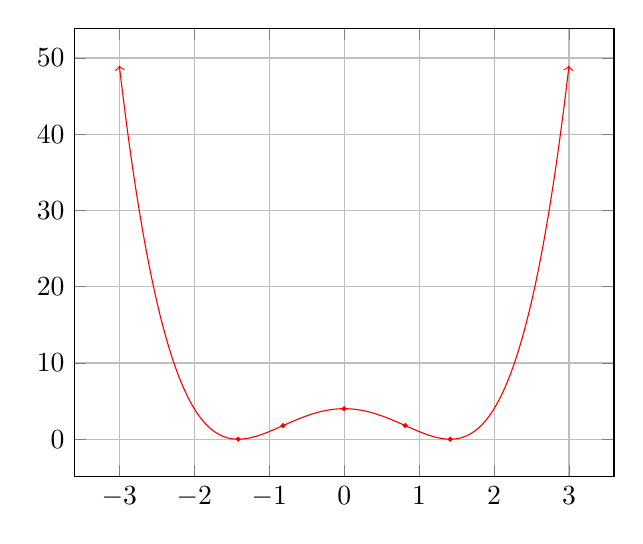
\begin{tikzpicture}
        \begin{axis}[domain=-3:3,
          samples=200,
          grid=both]
          \addplot[red,<->] { x^4-4*x^2+4 };
          \node[draw=red,fill=red,circle,inner sep=0.5pt]
          at (axis cs: -1.414,0) {};
          \node[draw=red,fill=red,circle,inner sep=0.5pt]
          at (axis cs: 0,4) {};
          \node[draw=red,fill=red,circle,inner sep=0.5pt]
          at (axis cs: 1.414,0) {};
          \node[draw=red,fill=red,circle,inner sep=0.5pt]
          at (axis cs: -0.816,1.778) {};
          \node[draw=red,fill=red,circle,inner sep=0.5pt]
          at (axis cs: 0.816,1.778) {};
        \end{axis}
      \end{tikzpicture}
      \caption{Graph of $y=x^4-4x^2+4$}
      \label{fig:x4-4x2+4}
    \end{figure}
  \item %1b
    \begin{itemize}
    \item[A] Domain: a polynomial has domain all of $\mathbb{R}$.
    \item[B] Intercepts: $x=0$ implies $y=(9-0^2)^3=729$.  $y=0$
      implies $(9-x^2)^3=0$ which implies $(9-x^2)=0$.  Factoring,
      $(3+x)(3-x)=0$ giving the $x$-intercepts $(-3,0)$ and $(3,0)$.
    \item[C] Symmetry: the function has only even powers of $x$, so it
      is an even function, with mirror symmetry in the $y$-axis; in
      other words, $y(-x)=y(x)$.
    \item[D] Asymptotes: non-constant polynomials do not have
      asymptotes.
    \item[E] Intervals of increase/decrease:
      $y'=3(9-x^2)^2(-2x)=-6(3+x)^2x(3-x)^2$.  The derivative is
      positive on $x<-3$, remains positive on $-3<x<0$, becomes
      negative on $0<x<3$, and remains negative on $3<x$.
    \item[F] Local max/min: the derivative only changes sign at $x=0$,
      which gives a local max.
    \item[G] Concavity and inflection points: the second derivative is
      \begin{align*}
        y'' &= 24(9-x^2)x^2-6(9-x^2)^2 = 6(9-x^2)(4x^2-9+x^2) \\
        &= 30(3+x)(x+3\sqrt{1/5})(x-3\sqrt{1/5})(3-x)
      \end{align*}
      which is negative on $x<-3$, positive on $-3<x<-3\sqrt{1/5}$,
      negative on $-3\sqrt{1/5}<x<3\sqrt{1/5}$, positive on
      $3\sqrt{1/5}<x<3$, and negative on $3<x$.  Since the concavity
      changes at each of the roots of $y''$, they are all inflection
      points.
    \item[H] Graph: see Figure~\ref{fig:9-x2all3}.
    \end{itemize}
    \begin{figure}[htbp]
      \centering
      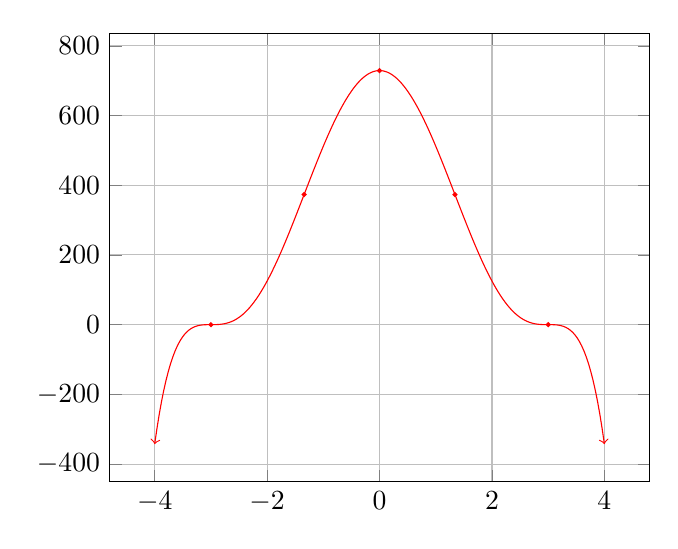
\begin{tikzpicture}
        \begin{axis}[domain=-4:4,
          samples=200,
          grid=both]
          \addplot[red,<->] { (9-x^2)^3  };
          \node[draw=red,fill=red,circle,inner sep=0.5pt]
          at (axis cs: -3,0) {};
          \node[draw=red,fill=red,circle,inner sep=0.5pt]
          at (axis cs: -1.342,373.248) {};
          \node[draw=red,fill=red,circle,inner sep=0.5pt]
          at (axis cs: 0,729) {};
          \node[draw=red,fill=red,circle,inner sep=0.5pt]
          at (axis cs: 1.342,373.248) {};
          \node[draw=red,fill=red,circle,inner sep=0.5pt]
          at (axis cs: 3,0) {};
        \end{axis}
      \end{tikzpicture}
      \caption{Graph of $y=(9-x^2)^3$}
      \label{fig:9-x2all3}
    \end{figure}
  \end{enumerate}
\item %2
  \begin{enumerate}
  \item %2a
    \begin{itemize}
    \item[A] Domain: rational functions are defined wherever the
      denominator is non-zero, so the domain is all of $\mathbb{R}$
      except for solutions to $9-x^2=0$ which are $x=-3$ and $x=3$.
    \item[B] Intercepts: when $x=0$, $y=0/9=0$.  When $y=0$,
      $x^2-3x=0$.  Factoring, $x(x-3)=0$ with roots $x=0$ and $x=3$.
      However, $x=3$ is not in the domain of the function, so the only
      $x$-intercept is at $x=0$.
    \item[C] Symmetry: there is no obvious relationship between $y(x)$
      and $y(-x)$ so there is no obvious symmetry.
    \item[D] Asymptotes:
      $\lim_{x\to\pm\infty} (x^2+3x)/(9-x^2) = \lim_{x\to\pm\infty}
      (1+3/x)/(9/x^2-1) = -1$, so the only horizontal asymptote is
      at $y=1$.  For vertical asymptotes, we take one-sided limits
      as $x$ approaches the locations at which the denominator is
      zero:
      \begin{align*}
        \lim_{x\to -3^-} \frac{x^2+3x}{9-x^2}
        &= \lim_{x\to -3^-} \frac{x(x+3)}{(3+x)(3-x)}
          = \lim_{x\to -3^-} \frac{x}{3-x} = \frac{-3}{6} = -\frac{1}{2} \\
        \lim_{x\to -3^+} \frac{x^2+3x}{9-x^2}
        &= \lim_{x\to -3^+} \frac{x(x+3)}{(3+x)(3-x)}
          = \lim_{x\to -3^+} \frac{x}{3-x} = \frac{-3}{6} = -\frac{1}{2} \\
        \lim_{x\to 3^-} \frac{x^2+3x}{9-x^2}
        &= \lim_{x\to 3^-} \frac{x(x+3)}{(3+x)(3-x)}
          = \lim_{x\to 3^-} \frac{x}{3-x} = \frac{3}{+0} = +\infty \\
        \lim_{x\to 3^+} \frac{x^2+3x}{9-x^2}
        &= \lim_{x\to 3^+} \frac{x(x+3)}{(3+x)(3-x)}
          = \lim_{x\to 3^+} \frac{x}{3-x} = \frac{3}{-0} = -\infty
      \end{align*}
      The only vertical asymptote is at $x=3$.  The function has a
      removable discontinuity at $x=-3$.
    \item[E] Intervals of increase/decrease: to simplify the
      calculation, remove the common factor of $x+3$ from the
      numerator and denominator and then apply the quotient rule:
      \begin{displaymath}
        y'=\frac{(3-x)-x(-1)}{(3-x)^2} = \frac{3}{(3-x)^2}
      \end{displaymath}
      The first derivative $y'$ is always positive on the domain of
      the function, so the function is increasing on its domain.
    \item[F] Local max/min: since $y'$ never changes sign, there are
      no local min/max.
    \item[G] Concavity and inflection points: by the chain rule the
      second derivative is
      \begin{displaymath}
        y'' = -6(3-x)^{-3}(-1) = 6(3-x)^{-3}
      \end{displaymath}
      The second derivative is positive for $x<3$, so concave up; the
      second derivative is negative for $x>3$, so concave down.  The
      only candidate for an inflection point would be at $x=3$ where
      the concavity changes, but $x=3$ is not in the domain of the
      function, so no inflection points.
    \item[H] Graph: see Figure~\ref{fig:x2+3xover9-x2}.
    \end{itemize}
    \begin{figure}[htbp]
      \centering
      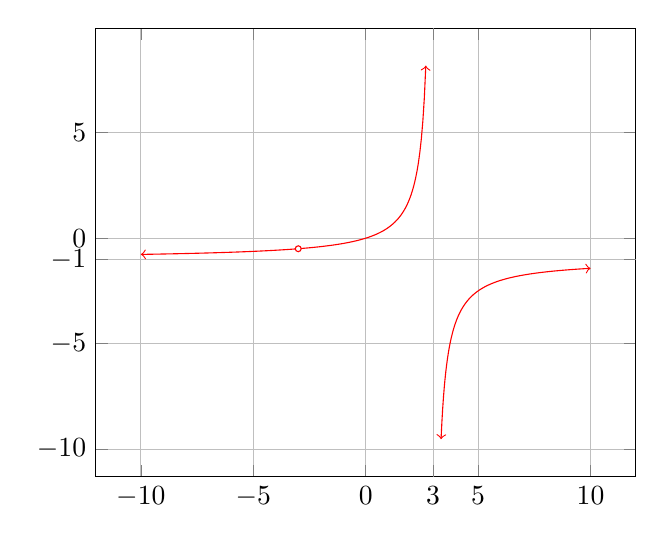
\begin{tikzpicture}
        \begin{axis}[domain=-10:10,
          restrict y to domain=-10:10,
          samples=200,
          extra x ticks=3,
          extra y ticks=-1,
          grid=both]
          \addplot[red,domain=-10:3,<->] { (x^2+3*x)/(9-x^2) };
          \addplot[red,domain=3:10,<->] { (x^2+3*x)/(9-x^2) };
          \node[draw=red,fill=white,circle,inner sep=0.75pt]
          at (axis cs:-3,-0.5) {};
        \end{axis}
      \end{tikzpicture}
      \caption{Graph of $\ds y=\frac{x^2+3x}{9-x^2}$}
      \label{fig:x2+3xover9-x2}
    \end{figure}
  \item %2b
    \begin{itemize}
    \item[A] Domain: the denominator is always positive, so the domain
      is all of $\mathbb{R}$.
    \item[B] Intercepts: when $x=0$, $y=(0-2)^2/(0^2+4)=4/4=1$, so
      $(0,1)$ is the $y$-intercept.  When $y=0$, $(x-2)^2/(x^+4)=0$
      which implies $(x-2)^2=0$ so $x=2$.  The point $(2,0)$ is the
      only $x$-intercept.
    \item[C] Symmetry: there is no obvious relationship between $y(x)$
      and $y(-x)$, so there is no obvious symmetry.
    \item[D] Asymptotes:
      \begin{displaymath}
        \lim_{x\to\pm\infty} \frac{(x-2)^2}{x^2+4}
        = \lim_{x\to\pm\infty} \frac{(x-2)^2/x^2}{(x^2+4)/x^2}
        = \lim_{x\to\pm\infty} \frac{(1-2/x)^2}{1+4/x^2}
        = \frac{(1-0)^2}{1+0} = 1
      \end{displaymath}
      so $y=1$ is the only horizontal asymptote.  Since the domain of
      this rational function is $\mathbb{R}$, there are no vertical
      asymptotes.
    \item[E] Intervals of increase/decrease: the derivative is
      \begin{align*}
        y' &= \frac{(x^2+4)\cdot 2(x-2) - (x-2)^2\cdot 2x}{(x^2+4)^2}
        = \frac{2x^3-4x^2+8x-16-2x^3+8x^2-8x}{(x^2+4)^2} \\
        &= \frac{4x^2-16}{(x^2+4)^2} = \frac{4(x+2)(x-2)}{(x^2+4)^2}
      \end{align*}
      The first derivative is positive for $x<-2$, negative for
      $-2<x<2$, and positive for $2<x$.
    \item[F] Local max/min: the derivative changes sign at $x=-2$
      (local max) and at $x=2$ (local min).
    \item[G] Concavity and inflection points: the second derivative is
      \begin{align*}
        y''
        &=\frac{(x^2+4)^2\cdot 8x - 4(x^2-4)\cdot 2(x^2+4)\cdot 2x}{(x^2+4)^4}
        \\
        &=\frac{(x^2+4)\cdot 8x - 4(x^2-4)\cdot 4x}{(x^2+4)^3}
        \\
        &= \frac{8x^3 + 32 x - 16x^3+64x}{(x^2+4)^3}
        \\
        &= \frac{-8x^3+96x}{(x^2+4)^3}
          = -\frac{8x(x+2\sqrt{3})(x-2\sqrt{3})}{(x^2+4)^3}
      \end{align*}
      The second derivative is positive on $x<-2\sqrt{3}$, negative on
      $-2\sqrt{3}<x<0$, positive on $0<x<2\sqrt{3}$, and negative on
      $2\sqrt{3}<x$.  Because the concavity changes at
      $x=-2\sqrt{3},0,2\sqrt{3}$, they are all inflection points.
    \item[H] Graph: see Figure~\ref{fig:x-2all2overx2+4}.
    \end{itemize}
    \begin{figure}[htbp]
      \centering
      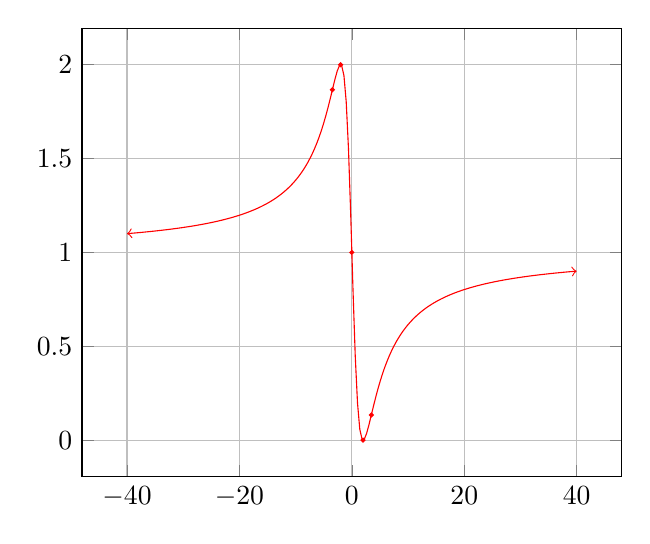
\begin{tikzpicture}
        \begin{axis}[domain=-40:40,
          restrict y to domain=-10:10,
          samples=200,
          %extra x ticks=3,
          %extra y ticks=-1,
          grid=both]
          \addplot[red,<->] { ((x-2)^2)/(x^2+4) };
          %\node[draw=red,fill=white,circle,inner sep=1pt]
          %at (axis cs:-3,-0.5) {};
          \node[draw=red,fill=red,circle,inner sep=0.5pt]
          at (axis cs: -3.464,1.866) {};
          \node[draw=red,fill=red,circle,inner sep=0.5pt]
          at (axis cs: -2,2) {};
          \node[draw=red,fill=red,circle,inner sep=0.5pt]
          at (axis cs: 0,1) {};
          \node[draw=red,fill=red,circle,inner sep=0.5pt]
          at (axis cs: 2,0) {};
          \node[draw=red,fill=red,circle,inner sep=0.5pt]
          at (axis cs: 3.464,0.134) {};
        \end{axis}
      \end{tikzpicture}
      \caption{Graph of $\ds y=\frac{(x-2)^2}{x^2+4}$}
      \label{fig:x-2all2overx2+4}
    \end{figure}
  \end{enumerate}
\item %3
  \begin{enumerate}
  \item\label{prob:sqrtx2+2x-x} %3a
    \begin{itemize}
    \item[A] Domain: the function is defined where the radicand
      $x^2+2x\ge 0$.  Factoring, we need $(x+2)x\ge 0$, which is true
      when both factors are negative or when both factors are
      positive, in other words, on $x\le -2$ and $0\le x$.
    \item[B] Intercepts: $x=0$ implies $y=\sqrt{0^2+2(0)}-0=0$, giving
      the $y$-intercept at $(0,0)$.  $y=0$ implies $\sqrt{x^2-2x}-x=0$
      which implies $\sqrt{x^2-2x}=x$ and $x^2-2x=x^2$ and finally
      $x=0$, so the only $x$-intercept is $(0,0)$.
    \item[C] Symmetry: there is no obvious relationship between $y(x)$
      and $y(-x)$ so there are no obvious symmetries.
    \item[D] Asymptotes: we evaluate the limit at infinity:
      \begin{align*}
        \lim_{x\to\infty} \sqrt{x^2+2x}-x
        &= \lim_{x\to\infty} (\sqrt{x^2+2x}-x)\cdot
          \frac{\sqrt{x^2+2x}+x}{\sqrt{x^2+2x}+x} \\
        &= \lim_{x\to\infty} \frac{x^2+2x-x^2}{\sqrt{x^2+2x}+x} \\
        &= \lim_{x\to\infty} \frac{2}{\sqrt{x^2+2x}/\sqrt{x^2}+1} \\
        &= \lim_{x\to\infty} \frac{2}{\sqrt{1+2/x}+1} \\
        &= \frac{2}{\sqrt{1+0}+1} = \frac{2}{2} = 1
      \end{align*}
      On the other hand, the limit at $-\infty$ is
      \begin{align*}
        \lim_{x\to -\infty} \sqrt{x^2+2x}-x
        &= \lim_{x\to -\infty} (\sqrt{x^2+2x}-x)\cdot
          \frac{\sqrt{x^2+2x}+x}{\sqrt{x^2+2x}+x} \\
        &= \lim_{x\to -\infty} \frac{x^2+2x-x^2}{\sqrt{x^2+2x}+x} \\
        &= \lim_{x\to -\infty} \frac{2}{-\sqrt{x^2+2x}/\sqrt{x^2}+1} \\
        &= \lim_{x\to -\infty} \frac{2}{-\sqrt{1+2/x}+1} \\
        &= \frac{2}{-\sqrt{1+0}+1} = \frac{2}{+0} = +\infty
      \end{align*}
      so there is no horizontal asymptote as $x\to -\infty$.  Note
      that a negative sign appears in the calculation because
      $x=-\sqrt{x^2}$ for negative $x$, and that the value of the
      denominator is positive $+0$ for large negative $x$ because
      $1+2/x<1$ for such $x$.  There are no vertical asymptotes
      because there is no denominator to go to $0$ in the function.
    \item[E] Intervals of increase/decrease: the derivative is
      \begin{displaymath}
        y'=\frac{1}{2}(x^2+2x)^{-1/2}\cdot (2x+2) - 1
        = \frac{x+1}{\sqrt{x^2+2x}} - 1
        = \frac{\pm\sqrt{x^2+2x+1}}{\sqrt{x^2+2x}} - 1
      \end{displaymath}
      For $0<x$, we use the $+$ sign in front of the square root, and
      then the fraction is always slightly larger than $0$ so $y'>0$,
      so $y$ is increasing.  For $x<-2$ we use the $-$ sign in front
      of the square root which makes $y'<0$, so $y$ is decreasing.
    \item[F] Local max/min: the first derivative does not change signs
      in the domain of the function so there are no local max/min in
      the interior of the domain.  There is a local min at both
      endpoints because in the neighborhood of $x=-2$ the function is
      decreasing and in the neighborhood of $x=0$ the function is
      increasing.
    \item[G] Concavity and inflection points: the second derivative is
      \begin{displaymath}
        y''=\frac{(x^2+2x)^{1/2}(1)- (x+1)\frac{1}{2}(x^2+2x)^{-1/2}(2x+2)}
        {x^2+2x}
        = \frac{x^2+2x-(x+1)^2}{(x^2+2x)^{3/2}}
        = -\frac{1}{(x^2+2x)^{3/2}}
      \end{displaymath}
      where we have simplified by multiplying the numerator and
      denominator by $(x^2+2x)^{1/2}$.  The second derivative is
      always negative so the graph is always concave down.
    \item[H] Graph: see Figure~\ref{fig:sqrtx2+2x-x}.
    \end{itemize}
    \begin{figure}[htbp]
      \centering
      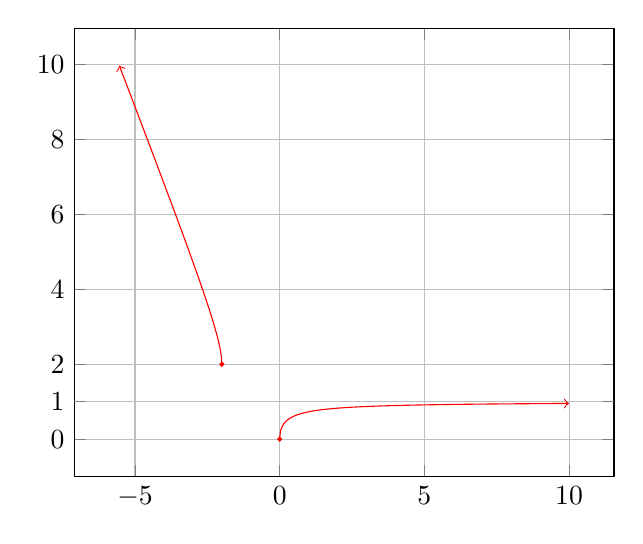
\begin{tikzpicture}
        \begin{axis}[domain=-10:10,
          restrict y to domain=-10:10,
          samples=500,
          %extra x ticks=3,
          extra y ticks=1,
          grid=both]
          \addplot[red,domain=-10:-2,<-] { sqrt(x^2+2*x)-x };
          \addplot[red,domain=0:10,->] { sqrt(x^2+2*x)-x };
          \node[draw=red,fill=red,circle,inner sep=0.5pt]
          at (axis cs: -2,2) {};
          \node[draw=red,fill=red,circle,inner sep=0.5pt]
          at (axis cs: 0,0) {};
          %\node[draw=red,fill=red,circle,inner sep=0.5pt]
          %at (axis cs: 0,1) {};
          %\node[draw=red,fill=red,circle,inner sep=0.5pt]
          %at (axis cs: 2,0) {};
          %\node[draw=red,fill=red,circle,inner sep=0.5pt]
          %at (axis cs: 3.464,0.134) {};
        \end{axis}
      \end{tikzpicture}
      \caption{Graph of $\ds y=\sqrt{x^2+2x}-x$}
      \label{fig:sqrtx2+2x-x}
    \end{figure}
  \item %3b
    \begin{itemize}
    \item[A] Domain: the radicand $x^2-4$ must be greater than $0$ so
      that the square root can be taken and so that the denominator is
      not $0$.  $x^2-4>0$ implies $(x+2)(x-2)>0$ which is true for
      $x<-2$ and $2<x$.
    \item[B] Intercepts: $x=0$ is not in the domain of the function so
      there is no $y$-intercept.  For $x$-intercepts,
      $x/\sqrt{x^2-4}=0$ implies $x=0$ which is again outside of the
      domain, so there are no $x$-intercepts.
    \item[C] Symmetry:
      $y(-x)=-x/\sqrt{(-x)^2-4}=-(x/\sqrt{x^2-4})=-y(x)$ so the
      function is odd, with rotational symmetry about the origin
      $(0,0)$.
    \item[D] Asymptotes: this function has interesting asymptotes.
      Taking the limit as $x\to\infty$ and dividing through by
      $x=\sqrt{x^2}$,
      \begin{displaymath}
        \lim_{x\to\infty} \frac{x}{\sqrt{x^2-4}}
        = \lim_{x\to\infty} \frac{x/x}{\sqrt{x^2-4}/\sqrt{x^2}}
        = \lim_{x\to\infty} \frac{1}{\sqrt{1-4/x^2}}
        = \frac{1}{\sqrt{1-0}}
        = 1
      \end{displaymath}
      Taking the limit as $x\to -\infty$ and dividing through by
      $x=-\sqrt{x^2}$,
      \begin{displaymath}
        \lim_{x\to -\infty} \frac{x}{\sqrt{x^2-4}}
        = \lim_{x\to -\infty} \frac{x/x}{-\sqrt{x^2-4}/\sqrt{x^2}}
        = \lim_{x\to -\infty} -\frac{1}{\sqrt{1-4/x^2}}
        = -\frac{1}{\sqrt{1-0}}
        = -1
      \end{displaymath}
      So this function has two different horizontal asymptotes, $y=1$
      and $y=-1$, which is a phenomenon that does not occur with
      rational functions.

      Candidates for vertical asymptotes are $x$-values at which the
      denominator of the function goes to $0$, namely $x=-2$ and
      $x=2$.  Those values are not in the domain of the function, but
      we can still take one-sided limits as $x$ approaches those
      values:
      \begin{align*}
        \lim_{x\to -2^-} \frac{x}{\sqrt{x^2-4}} &= \frac{-2}{+0} = -\infty
        \\
        \lim_{x\to 2^+} \frac{x}{\sqrt{x^2-4}} &= \frac{2}{+0} = +\infty
      \end{align*}
      which show that both $x=-2$ and $x=2$ are vertical asymptotes.
    \item[E] Intervals of increase/decrease: the derivative is
      \begin{displaymath}
        y'=\frac{(x^2-4)^{1/2}(1)-x\cdot\frac{1}{2}(x^2-4)^{-1/2}(2x)}{x^2-4}
        = \frac{x^2-4-x^2}{(x^2-4)^{3/2}} = -\frac{4}{(x^2-4)^{3/2}}
      \end{displaymath}
      which is always negative so the function is always decreasing.
    \item[F] Local max/min: since the function is always decreasing,
      there can be no local max/min.
    \item[G] Concavity and inflection points: the second derivative is
      \begin{displaymath}
        y'' = 6(x^2-4)^{-5/2}\cdot 2x
      \end{displaymath}
      which has the same sign as $x$, so the function is concave down
      for $x<-2$ and concave up for $2<x$.
    \item[H] Graph: see Figure~\ref{fig:xoversqrtx2-4}.
    \end{itemize}
    \begin{figure}[htbp]
      \centering
      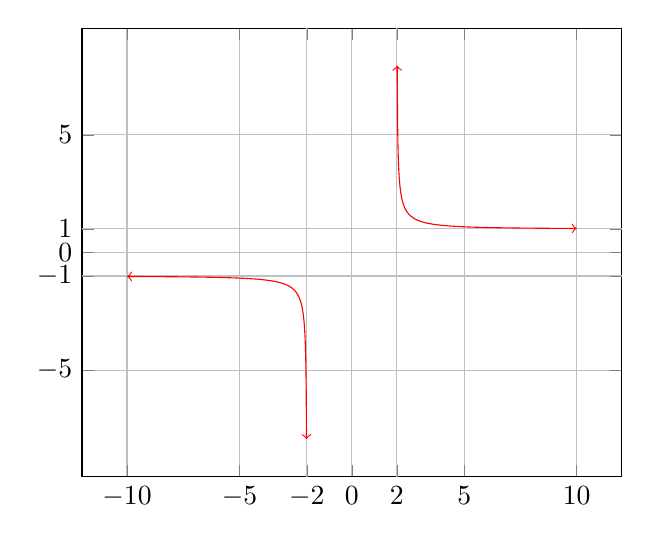
\begin{tikzpicture}
        \begin{axis}[domain=-10:10,
          restrict y to domain=-10:10,
          samples=500,
          extra x ticks={-2,2},
          extra y ticks={-1,1},
          grid=both]
          \addplot[red,domain=-10:-2,<->] { x/sqrt(x^2-4) };
          \addplot[red,domain=2:10,<->] { x/sqrt(x^2-4) };
        \end{axis}
      \end{tikzpicture}
      \caption{Graph of $\ds y=\frac{x}{\sqrt{x^2-4}}$}
      \label{fig:xoversqrtx2-4}
    \end{figure}    
  \end{enumerate}
\item %4
  \begin{enumerate}
  \item %4a
    \begin{itemize}
    \item[A] Domain: the domain is given in the problem statement:
      $[-2\pi,2\pi]$.
    \item[B] Intercepts: when $x=0$, $y=0+\sin 0=0+0=0$, so $(0,0)$ is
      the $y$-intercept.  For the $x$-intercept we need to solve
      $0=x+\sin x$.  Solving such trigonometric equations can be
      difficult, but we have done most of the work already in Problem
      Set~3.2 where we used the mean value theorem to show that
      $|\sin x|\le |x|$ for all $x$.  A slight refinement of the
      solutions to Problem Set~3.2 shows that $|\sin x|<|x|$ for
      $-2\pi\le x<0$ and for $0<x\le 2\pi$.  So the only possible
      solution in our domain is $x=0$, and a quick check shows that
      $x=0$ is a solution.
    \item[C] Symmetry: we have $y(-x)=-x+\sin(-x)=-x-\sin x=-y(x)$ so
      the function is odd, with rotational symmetry about the origin
      $(0,0)$.
    \item[D] Asymptotes: the domain is finite so there are no
      horizontal asymptotes.  The values of the function are bounded
      on its domain (because $-2\pi-1\le x+\sin x\le 2\pi+1$ so there
      are no vertical asymptotes.
    \item[E] Intervals of increase/decrease: the derivative is
      \begin{displaymath}
        y' = 1 + \cos x
      \end{displaymath}
      Since $-1\le \cos x \le 1$, it follows that $y'\ge 0$, and the
      function is non-decreasing.
    \item[F] Local max/min: the points where $y'=0$ are solutions to
      $\cos x = -1$, which we know from the graph of cosine are
      $x=-\pi$ and $x=\pi$.  (There are more solutions: $x=k\pi$,
      where $k$ is an odd integer, but $\pm\pi$ are the only solutions
      in the domain $[-2\pi,2\pi]$.)  However, the derivative does not
      change sign at $\pm\pi$, so they are not locations of local
      max/min.  Since the function is defined on a finite interval,
      the endpoints are candidates for local max/min: $x=-2\pi$ is a
      local min because the function is increasing in its
      neighborhood, and similarly $x=2\pi$ is a local max because the
      function is increasing in its neighborhood.
    \item[G] Concavity and inflection points: the second derivative is
      $y''=-\sin x$, which one can easily graph to obtain $y''<0$ on
      the interval $-2\pi<x<-\pi$, $y''>0$ on the interval $-\pi<x<0$,
      $y''<0$ on the interval $0<x<\pi$, and $y''<0$ on the interval
      $\pi<x<2\pi$.  Since the concavity changes at each of
      $x=-\pi,0,\pi$, those are all inflection points.
    \item[H] Graph:
    \end{itemize}
    \begin{figure}[htbp]
      \centering
      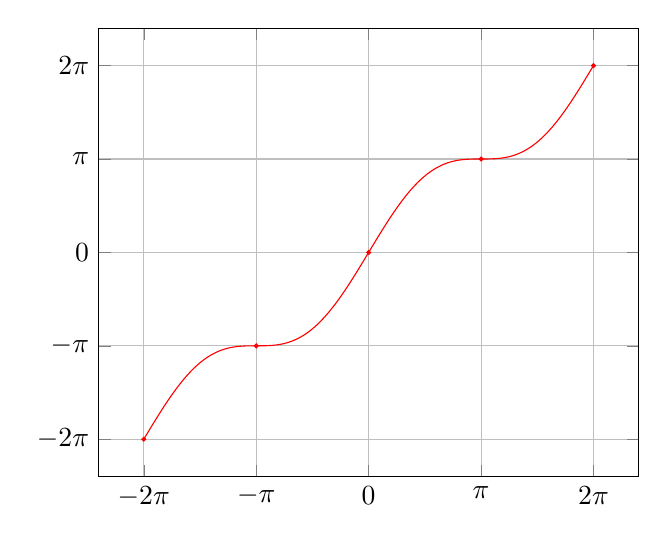
\begin{tikzpicture}
        \begin{axis}[domain=-2*pi:2*pi,
          %restrict y to domain=-10:10,
          samples=500,
          %extra x ticks={-2,2},
          %extra y ticks={-1,1},
          ytick={-2*pi, -pi, 0, pi, 2*pi},
          yticklabels={
            $-2\pi$, $-\pi$, $0$, $\pi$, $2\pi$ },
          xtick={-2*pi, -pi, 0, pi, 2*pi},
          xticklabels={
            $-2\pi$, $-\pi$, $0$, $\pi$, $2\pi$ },
          grid=both]
          \addplot[red,domain=-2*pi:2*pi] { x + sin(deg(x)) };
          \node[draw=red,fill=red,circle,inner sep=0.5pt]
          at (axis cs: -2*pi,-2*pi) {};
          \node[draw=red,fill=red,circle,inner sep=0.5pt]
          at (axis cs: -pi,-pi) {};
          \node[draw=red,fill=red,circle,inner sep=0.5pt]
          at (axis cs: 0,0) {};
          \node[draw=red,fill=red,circle,inner sep=0.5pt]
          at (axis cs: pi,pi) {};
          \node[draw=red,fill=red,circle,inner sep=0.5pt]
          at (axis cs: 2*pi,2*pi) {};
        \end{axis}
      \end{tikzpicture}
      \caption{Graph of $\ds y=x+\sin x$}
      \label{fig:x+sinx}
    \end{figure}    
  \item %4b
    \begin{itemize}
    \item[A] Domain: the function is defined on $\mathbb{R}$ except
      where the denominator is $0$.  However, $-1\le \cos x \le 1$ for
      all $x$, so $2+\cos x$ is never $0$.
    \item[B] Intercepts: when $x=0$, $y=\sin(0)/(2+\cos(0))=0/3=0$ so
      the $y$-intercept is $(0,0)$.  When $y=0$, $\sin x/(2+\cos x)=0$
      which implies $\sin x =0$.  From a graph of $\sin x$ we see that
      the solutions are at $x=k\pi$ where $k$ is any integer.  So
      there are $x$-intercepts at the points $(k\pi,0)$ where $k$ is
      any integer.
    \item[C] Symmetry: there is no obvious relationship between $y(x)$
      and $y(-x)$ so there is no obvious mirror or rotational
      symmetry.  However, with trigonometric functions we often see
      another kind of symmetry, ``translational'' symmetry, also
      called ``periodicity''.  In this case
      \begin{displaymath}
        y(x+2\pi)=\frac{\sin(x+2\pi)}{2+\cos(x+2\pi)}
        = \frac{\sin x}{2+\cos x} = y(x)
      \end{displaymath}
      so the function is periodic with period $2\pi$.  We only have to
      graph a single period of the function to get a complete picture
      of its behaviour (but we will graph several periods below so
      that we can see what periodicity means geometrically).
    \item[D] Asymptotes: because of periodicity, there are no
      horizontal asymptotes.  Because the denominator never goes to
      $0$ there are no vertical asymptotes.
    \item[E] Intervals of increase/decrease: the first derivative is
      \begin{displaymath}
        y'=\frac{(2+\cos x)\cdot \cos x - \sin x (-\sin x)}{(2+\cos x)^2}
        = \frac{2\cos x +\cos^2 x + \sin^2 x}{(2+\cos x)^2}
        = \frac{2\cos x + 1}{(2+\cos x)^2}
      \end{displaymath}
      where we have used the Pythagorean identity to simplify in the
      last step.  The sign of the derivative is the same as the sign
      of $2\cos x+1$.  To find where it changes sign we solve
      $2\cos x+1=0$ which is equivalent to $\cos x = -1/2$.  From our
      knowledge of trigonometric functions we have solutions
      $x=\pm 2\pi/3+ 2k\pi$; in other words, $2\cos x + 1$ is positive
      for $0\le x < 2\pi/3$, negative on $2\pi/3 < x < 4\pi/3$,
      positive on $4\pi/3<x\le 2\pi$, and the pattern recurs with a
      period of $2\pi$.
    \item[F] Local max/min: the first derivative goes from positive to
      negative at $x=2\pi/3$ so there is a local max there (and
      consequently at every $x$ value of the form $2\pi/3+2k\pi$ where
      $k$ is an integer).  The first derivative goes from negative to
      positive at $x=4\pi/3$ so there is a local min there (and
      consequently at ever $x$ value of the form $4\pi/3+2k\pi$ where
      $k$ is an integer).
    \item[G] Concavity and inflection points: the second derivative is
      \begin{align*}
        y'' &= \frac{(2+\cos x)^2 \cdot 2(-\sin x)
              - (2\cos x+1)\cdot 2(2+\cos x)(-\sin x)}{(2+\cos x)^4}
        \\
            &= \frac{-8\sin x -8 \sin x \cos x - 2\sin x\cos^2 x
              + 8 \sin x \cos x + 4 \sin x \cos^2 x + 4\sin x + 2\sin x\cos x}
              {(2+\cos x)^4}
        \\
            &= \frac{-4\sin x + 2\sin x\cos^2 x + 2\sin x \cos x}{(2+\cos x)^4}
        \\
            &= \frac{2\sin x(\cos^2 x + \cos x - 2)}{(2+\cos x)^4}
        \\
            &= \frac{2\sin x(\cos x +2)(\cos x -1)}{(2+\cos x)^4}
        \\
            &= \frac{2\sin x(\cos x -1)}{(2+\cos x)^3}
      \end{align*}
      The second derivative is $0$ whenever $\sin x=0$ or $\cos x =1$.
      The solutions to those equations are actually the same, namely
      $x=k\pi$ where $k$ is an integer, so those are our potential
      points of inflection.  Note that $\cos x - 1\le 0$ and
      $2+\cos x>0$ so the sign of the second derivative depends on
      $\sin x$ only; the latter goes from negative to positive at
      $x=0$, from positive to negative at $x=\pi$, and so on, so all
      the potential inflection points are actual inflection points.
    \item[H] Graph: see Figure~\ref{fig:sinxover2+cosx}.
    \end{itemize}
    \begin{figure}[htbp]
      \centering
      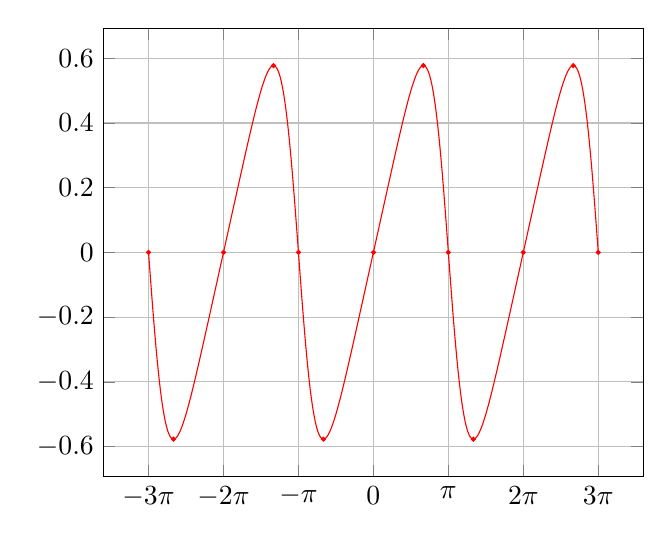
\begin{tikzpicture}
        \begin{axis}[domain=-3*pi:3*pi,
          samples=500,
          xtick={-3*pi, -2*pi, -pi, 0, pi, 2*pi, 3*pi},
          xticklabels={$-3\pi$, $-2\pi$, $-\pi$, $0$, $\pi$, $2\pi$, $3\pi$},
          grid=both]
          \addplot[red] { sin(deg(x))/(2+cos(deg(x))) };
          \node[draw=red,fill=red,circle,inner sep=0.5pt]
          at (axis cs: -3*pi,0) {};
          \node[draw=red,fill=red,circle,inner sep=0.5pt]
          at (axis cs: -2*pi,0) {};
          \node[draw=red,fill=red,circle,inner sep=0.5pt]
          at (axis cs: -pi,0) {};
          \node[draw=red,fill=red,circle,inner sep=0.5pt]
          at (axis cs: 0,0) {};
          \node[draw=red,fill=red,circle,inner sep=0.5pt]
          at (axis cs: 3*pi,0) {};
          \node[draw=red,fill=red,circle,inner sep=0.5pt]
          at (axis cs: 2*pi,0) {};
          \node[draw=red,fill=red,circle,inner sep=0.5pt]
          at (axis cs: pi,0) {};
          \node[draw=red,fill=red,circle,inner sep=0.5pt]
          at (axis cs: 2*pi/3,0.57735) {};  % sqrt(3)/3
          \node[draw=red,fill=red,circle,inner sep=0.5pt]
          at (axis cs: 8*pi/3,0.57735) {};  % sqrt(3)/3
          \node[draw=red,fill=red,circle,inner sep=0.5pt]
          at (axis cs: -4*pi/3,0.57735) {};  % sqrt(3)/3
          \node[draw=red,fill=red,circle,inner sep=0.5pt]
          at (axis cs: -2*pi/3,-0.57735) {};  % sqrt(3)/3
          \node[draw=red,fill=red,circle,inner sep=0.5pt]
          at (axis cs: -8*pi/3,-0.57735) {};  % sqrt(3)/3
          \node[draw=red,fill=red,circle,inner sep=0.5pt]
          at (axis cs: 4*pi/3,-0.57735) {};  % sqrt(3)/3
        \end{axis}
      \end{tikzpicture}
      \caption{Graph of $\ds y=\frac{\sin x}{2+\cos x}$}
      \label{fig:sinxover2+cosx}
    \end{figure}    
  \end{enumerate}
\item %5
  The functions both are rational with numerator of degree one higher
  than denominator, so they should both have slant asymptotes.  We do
  polynomial division to find those slant asymptotes.
  \begin{enumerate}
  \item %5a
    By polynomial division,
    \begin{displaymath}
      5x^2-7x+8 = (x-3)(5x+8)+32
    \end{displaymath}
    so
    \begin{displaymath}
      \frac{5x^2-7x+8}{x-3} = 5x+8 + \frac{32}{x-3}
      \implies
      \lim_{x\to\pm\infty} \frac{5x^2-7x+8}{x-3}-(5x+8)
      = \lim_{x\to\pm\infty}\frac{32}{x-3} = 0
    \end{displaymath}
    It follows that the slant asymptote is $y=5x+8$.
  \item %5b
    By polynomial division,
    \begin{displaymath}
      2x^3-4x^2+5 = (x^2-3x-1)(2x+2) + 8x +7
    \end{displaymath}
    so
    \begin{displaymath}
      \lim_{x\to\pm\infty} \frac{2x^3-4x^2+5}{x^2-3x-1} - (2x+2)
      = \lim_{x\to\pm\infty} \frac{8x+7}{x^2-3x-1}
      = 0
    \end{displaymath}
    and $y=2x+2$ is the slant asymptote.
  \end{enumerate}
\item %6
  We follow the same set of steps as always, except we look for slant
  asymptotes instead of horizontal asymptotes in step D.
  \begin{enumerate}
  \item %6a
    \begin{itemize}
    \item[A] Domain: the domain of the rational function is all real
      numbers except those where the denominator is $0$, namely
      $x=-2$.
    \item[B] Intercepts: when $x=0$, $y=1/2$.  When $y=0$,
      $1-2x-3x^2=0$.  Factoring, $(1+x)(1-3x)=0$ which gives
      $x$-intercepts at $(-1,0)$ and $(1/3,0)$.
    \item[C] Symmetry: there is no obvious relationship between $y(x)$
      and $y(-x)$ so no obvious symmetry.
    \item[D] Asymptotes: since the degree of the numerator is one more
      than the degree of the denominator, there is no horizontal
      asymptote, but there may be a slant asymptote.  By polynomial
      division,
      \begin{displaymath}
        1-2x-3x^2 = (x+2)(-3x + 4) -7
      \end{displaymath}
      so
      \begin{displaymath}
        \frac{1-2x-3x^2}{x+2} = -3x + 4 - \frac{7}{x+2}
        \implies
        \lim_{x\to\pm\infty} \frac{1-2x-3x^2}{x+2} - (-3x+4)
        = \lim_{x\to\pm\infty} -\frac{7}{x+2} = 0
      \end{displaymath}
      so the slant asymptote is $y=-3x+4$.

      There is also a vertical asymptote at $x=-2$ because
      \begin{displaymath}
        \lim_{x\to -2^-} \frac{1-2x-3x^2}{x+2}
        = \lim_{x\to -2^-} \frac{(1+x)(1-3x)}{x+2}
        = \frac{(-1)(7)}{-0} = +\infty
      \end{displaymath}
      and
      \begin{displaymath}
        \lim_{x\to -2^+} \frac{1-2x-3x^2}{x+2}
        = \lim_{x\to -2^+} \frac{(1+x)(1-3x)}{x+2}
        = \frac{(-1)(7)}{+0} = -\infty
      \end{displaymath}
    \item[E] Intervals of increase/decrease: the derivative is
      \begin{align*}
        y'&=\frac{(x+2)(-2-6x)-(1-2x-3x^2)(1)}{(x+2)^2}
        = \frac{-2x-6x^2-4-12x-1+2x+3x^2}{(x+2)^2} \\
        &= \frac{-3x^2-12x-5}{(x+2)^2} 
      \end{align*}
      The roots of the quadratic in the numerator can be found using
      the quadratic formula:
      \begin{displaymath}
        x= -2 \pm \sqrt{\frac{7}{3}}
      \end{displaymath}
      The numerator is negative to the left of the first root ($y$ is
      decreasing), is positive between the roots ($y$ is increasing),
      and is negative to the right of the second root ($y$ is
      decreasing).
    \item[F] Local max/min: since the derivative changes sign at its
      two roots, they are a local min and local max respectively.
    \item[G] Concavity and inflection points: after some calculation,
      the second derivative is
      \begin{displaymath}
        y''= -\frac{14}{(x+2)^3}
      \end{displaymath}
      which has the opposite sign of $x+2$, so the function is concave
      up on $x<-2$ and concave down on $-2<x$.  The point $x=-2$ is
      not an inflection point because the function is not defined
      there.
    \item[H] Graph: see Figure~\ref{fig:1-2x-3x2overx+2}.
    \end{itemize}
    \begin{figure}[htbp]
      \centering
      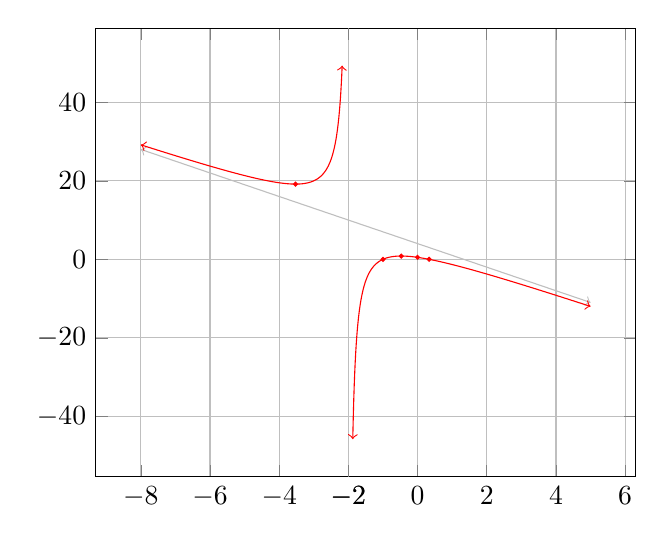
\begin{tikzpicture}
        \begin{axis}[domain=-8:5,
          restrict y to domain=-50:50,
          samples=500,
          extra x ticks=-2,
          %extra y ticks=-1,
          grid=both]
          \addplot[lightgray,domain=-8:5,<->] { (-3*x+4) };
          \addplot[red,domain=-8:-2,<->] { (1-2*x-3*x^2)/(x+2) };
          \addplot[red,domain=-2:5,<->]  { (1-2*x-3*x^2)/(x+2) };
          %\node[draw=red,fill=white,circle,inner sep=1pt]
          %at (axis cs:-3,-0.5) {};
          \node[draw=red,fill=red,circle,inner sep=0.5pt]
          at (axis cs: 0,0.5) {};
          \node[draw=red,fill=red,circle,inner sep=0.5pt]
          at (axis cs: -1,0) {};
          \node[draw=red,fill=red,circle,inner sep=0.5pt]
          at (axis cs: 0.33333,0) {};
          \node[draw=red,fill=red,circle,inner sep=0.5pt]
          at (axis cs: -3.52753,19.1652) {};
          \node[draw=red,fill=red,circle,inner sep=0.5pt]
          at (axis cs: -0.472475,0.834849) {};          
        \end{axis}
      \end{tikzpicture}
      \caption{Graph of $\ds y=\frac{1-2x-3x^2}{x+2}$}
      \label{fig:1-2x-3x2overx+2}
    \end{figure}
  \item %6b
    \begin{itemize}
    \item[A] Domain: the domain of this rational function is all of
      $\mathbb{R}$ except for $x$ values where the denominator is $0$,
      namely $x=-2$.
    \item[B] Intercepts: $x=0$ implies $y=-8/4=-2$.  $y=0$ implies
      $(x-2)^3=0$ with solution $x=2$.
    \item[C] Symmetry: there is no obvious relationship between $y(x)$
      and $y(-x)$, so no obvious symmetry.
    \item[D] Asymptotes: since the degree of the numerator is one more
      than the degree of the denominator, there is no horizontal
      asymptote, but there may be a slant asymptote.  By polynomial
      division,
      \begin{displaymath}
        x^3-2x^2+4x-8 = (x^2+4x+4)(x-6) + 24x+16
      \end{displaymath}
      By a calculation similar to that of the previous problem, the
      slant asymptote is $y=x-6$.  There is a potential vertical
      asymptote at $x=-2$ which we can easily verify by taking limits:
      \begin{align*}
        \lim_{x\to -2^-} \frac{(x-2)^3}{(x+2)^2} &= \frac{-64}{+0} = -\infty
        \\
        \lim_{x\to -2^+} \frac{(x-2)^3}{(x+2)^2} &= \frac{-64}{+0} = -\infty
      \end{align*}
    \item[E] Intervals of increase/decrease: the derivative is
      \begin{displaymath}
        y' = \frac{(x+2)^2\cdot 3(x-2)^2 - (x-2)^3\cdot 2(x+2)}{(x+2)^4}
        = \frac{(x-2)^2(3(x+2)-2(x-2))}{(x+2)^3}
        = \frac{(x-2)^2(x+10)}{(x+2)^3}
      \end{displaymath}
      The sign of $y'$ changes from positive to negative at $x=-10$,
      and then changes from negative to positive at $x=-2$.  It then
      goes to $0$ at $x=2$ but stays positive for $2<x$.  The function
      increases on $x<-10$, decreases on $-10<x<-2$, increases on
      $-2<x<2$, and increases on $2<x$.
    \item[F] Local max/min: since the derivative changes sign from
      positive to negative at $x=-10$ there is a local max there.
      There is no local min at $x=-2$ because the function is not
      defined there.  There is no local max/min at $x=2$ because the
      derivative does not change sign there.
    \item[G] Concavity and inflection points: after some calculating,
      \begin{displaymath}
        y''=\frac{96(x-2)}{(x+2)^4}
      \end{displaymath}
      which is negative (concave down) for $x<2$ and positive (concave
      up) for $2<x$.
    \item[H] Graph: see Figure~\ref{fig:x-2all3overx+2all2}.
    \end{itemize}
  \end{enumerate}
  \begin{figure}[htbp]
    \centering
    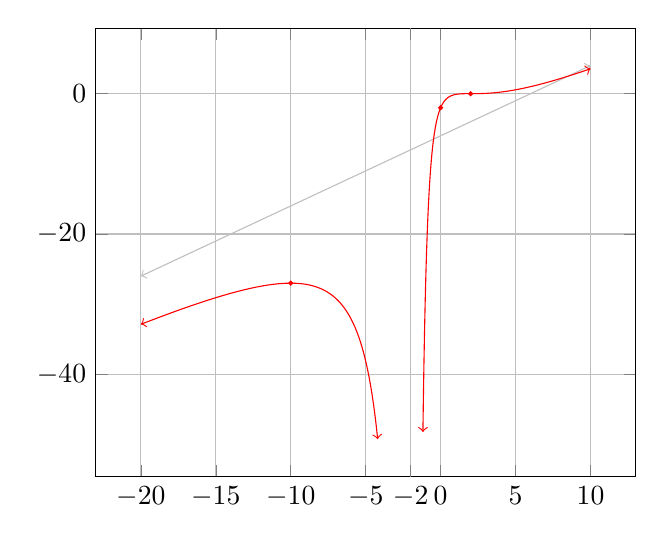
\begin{tikzpicture}
      \begin{axis}[domain=-20:10,
        restrict y to domain=-50:10,
        samples=500,
        extra x ticks=-2,
          %extra y ticks=-1,
        grid=both]
        \addplot[lightgray,domain=-20:10,<->] { (x-6) };
        \addplot[red,domain=-20:-2,<->] { ((x-2)^3)/(x+2)^2 };
        \addplot[red,domain=-2:10,<->] { ((x-2)^3)/(x+2)^2 };
        \node[draw=red,fill=red,circle,inner sep=0.5pt]
        at (axis cs:0,-2) {};
        \node[draw=red,fill=red,circle,inner sep=0.5pt]
        at (axis cs: 2,0) {};
        \node[draw=red,fill=red,circle,inner sep=0.5pt]
        at (axis cs: -10,-27) {};
      \end{axis}
    \end{tikzpicture}
    \caption{Graph of $\ds y=\frac{(x-2)^3}{(x+2)^2}$}
    \label{fig:x-2all3overx+2all2}
  \end{figure}
\item %7
  This problem is similar to the other graphing problems we have done,
  except that it involves the parameters $m_0$ and $c$ instead of just
  numbers.
  \begin{itemize}
  \item[A] Domain: the radicand $1-v^2/c^2$ must be greater than $0$
    for the function to be defined; $1-v^2/c^2>0$ implies $v^2<c^2$,
    or in other words, $-c<v<c$.
  \item[B] Intercepts: when $v=0$, $m=m_0$.  It is not possible to
    have $m=0$ (unless $m_0=0$, which is an uninteresting special
    case).
  \item[C] Symmetry:
    $m(-v)=m_0/\sqrt{1-(-v)^2/c^2}=m_0/\sqrt{1-v^2/c^2}=m(v)$ so the
    function has mirror symmetry in the $y$-axis.
  \item[D] Asymptotes: the domain is bounded, so there can be no
    horizontal or slant asymptotes.  The denominator goes to $0$ when
    $v\to\pm c$ so there may be vertical asymptotes at $v=\pm c$.
    Checking the relevant limits,
    \begin{align*}
      \lim_{v\to -c^+} \frac{m_0}{\sqrt{1-v^2/c^2}} &= \frac{m_0}{+0} = +\infty
      \\
      \lim_{v\to c^-} \frac{m_0}{\sqrt{1-v^2/c^2}} &= \frac{m_0}{+0} = +\infty
    \end{align*}
  \item[E] Intervals of increase/decrease: the derivative is
    \begin{displaymath}
      y'=m_0\cdot -\frac{1}{2} (1-v^2/c^2)^{-3/2} \cdot -2v/c^2
      = \frac{m_0v}{c^2(1-v^2/c^2)^{3/2}}
    \end{displaymath}
    which has the same sign as $v$, $m(v)$ is decreasing on $-c<v<0$
    and increasing on $0<v<c$.
  \item[F] Local max/min: the derivative changes sign from negative to
    positive at $v=0$, so that is a local min.
  \item[G] Concavity and inflection points: the second derivative is
    \begin{align*}
      y''&=\frac{m_0}{c^2} \left( (1-v^2/c^2)^{-3/2} + v \cdot -\frac{3}{2}
        (1-v^2/c^2)^{-5/2} \cdot -2v/c^2 \right) \\
      &= \frac{m_0}{c^2} \left( (1-v^2/c^2) + 3 v^2/c^2 \right)
      (1-v^2/c^2)^{-5/2} \\
      &=\frac{m_0}{c^2} \frac{1+2v^2/c^2}{(1-v^2/c^2)^{5/2}}
    \end{align*}
    The second derivative is always positive so the function is
    concave up everywhere in its domain.
  \item[H] Graph: see Figure~\ref{fig:relativity}.
  \end{itemize}
  \begin{figure}[htbp]
    \centering
    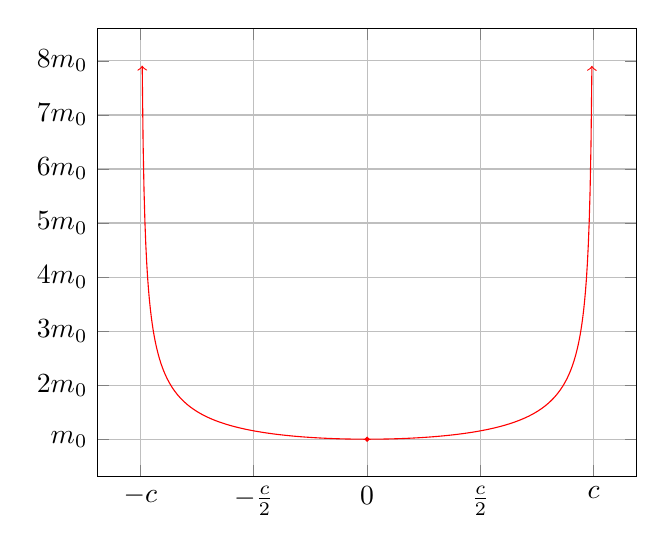
\begin{tikzpicture}
      \begin{axis}[domain=-1:1,
        restrict y to domain=-10:10,
        xtick={-1, -0.5, 0, 0.5, 1},
        xticklabels={$-c$, $-\frac{c}{2}$, $0$, $\frac{c}{2}$, $c$},
        ytick={0,1,2,3,4,5,6,7,8,9,10},
        yticklabels={$0$,$m_0$,$2m_0$,$3m_0$,$4m_0$,$5m_0$,$6m_0$,$7m_0$,
          $8m_0$, $9m_0$, $10m_0$},
        samples=500,
        grid=both]
        \addplot[red,domain=-1:1,<->] { 1/sqrt(1-x^2) };
        \node[draw=red,fill=red,circle,inner sep=0.5pt]
        at (axis cs: 0,1) {};
      \end{axis}
    \end{tikzpicture}
    \caption{Graph of $\ds m=\frac{m_0}{\sqrt{1-v^2/c^2}}$}
    \label{fig:relativity}
  \end{figure}    
\item %8
  The slant asymptotes are checked in step D below.
  \begin{itemize}
  \item[A] Domain: the radicand must be greater than or equal to $0$,
    so $x^2-4x\ge 0$.  Factoring, $x(x-4)\ge 0$ which is true when
    $x\le 0$ or when $4\ge x$.
  \item[B] Intercepts: $x=0$ implies $y=0$.  $y=0$ implies $x^2-4x=0$
    with solutions $x=0$, $x=4$.
  \item[C] Symmetry: there is no obvious relationship between $y(x)$
    and $y(-x)$ so there is no obvious symmetry.
  \item[D] Asymptotes: as suggested, we will investigate two potential
    slant asymptotes by taking the limit as $x\to\pm\infty$ of the
    difference between the function and the proposed asymptote.  In
    the limit calculation, we will multiply and divide by conjugate
    radicals.
    \begin{align*}
      \lim_{x\to\infty} \sqrt{x^2-4x}-(x-2)
      &= \lim_{x\to\infty} \left(\sqrt{x^2-4x}-(x-2)\right)
        \cdot\frac{\sqrt{x^2-4x}+(x-2)}{\sqrt{x^2-4x}+(x-2)} \\
      &= \lim_{x\to\infty} \frac{x^2-4x - x^2 + 4x - 4}{\sqrt{x^2-4x}+(x-2)} \\
      &= \lim_{x\to\infty} \frac{-4}{\sqrt{x^2-4x}+(x-2)}
        = \frac{4}{\infty} =0
    \end{align*}
    which shows that $y=x-2$ is a slant asymptote as $x\to\infty$.
    The limit as $x\to -\infty$ is similar:
    \begin{align*}
      \lim_{x\to -\infty} \sqrt{x^2-4x}-(-x+2)
      &= \lim_{x\to -\infty} \left(\sqrt{x^2-4x}-(-x+2)\right)
        \cdot\frac{\sqrt{x^2-4x}+(-x+2)}{\sqrt{x^2-4x}+(-x+2)} \\
      &= \lim_{x\to -\infty} \frac{x^2-4x-x^2+4x-4}{\sqrt{x^2-4x}+(-x+2)} \\
      &= \lim_{x\to -\infty} \frac{-4}{\sqrt{x^2-4x}+(-x+2)}
        = \frac{4}{\infty} =0        
    \end{align*}
    where in the last line we have used $-x$ is positive.  (If we had
    used $x-2$ instead of $-x+2$ in this calculation, the
    $\sqrt{x^2-4x}$ and $x-2$ in the denominator would cancel and we
    would not get the denominator tending to $\infty$.)  That shows
    that $y=-x+2$ is a slant asymptote as $x\to -\infty$.
  \item[E] Intervals of increase/decrease: the derivative is
    \begin{displaymath}
      y' = \frac{1}{2} (x^2-4x)^{-1/2} \cdot (2x-4) = \frac{x-2}{\sqrt{x^2-4x}}
    \end{displaymath}
    which has the same sign as $x-2$ so the function is decreasing on
    $x<0$ and increasing on $4<x$.
  \item[F] Local max/min: the derivative does not change sign in the
    domain so there are no local max/min except for the endpoints of
    the domain, $x=0$ and $x=4$, which are both local minimums.
  \item[G] Concavity and inflection points: the second derivative of
    the function is
    \begin{displaymath}
      y''=(x^2-4x)^{-1/2}
      + (x-2) \cdot -\frac{1}{2} (x^2-4x)^{-3/2} \cdot (2x-4)
      = \frac{x^2-4x - (x-2)^2}{(x^2-4x)^{3/2}}
      = -\frac{4}{(x^2-4x)^{3/2}}
    \end{displaymath}
    which is always negative so the function is always concave down.
  \item[H] Graph: see Figure~\ref{fig:sqrtx2-4x}.
  \end{itemize}
  Now that we have a new technique for checking slant asymptotes, you
  should go back to Problem~\ref{prob:sqrtx2+2x-x} to try to figure
  out what the slant asymptote is, and then to check it by taking the
  limit $x\to -\infty$.
  \begin{figure}[htbp]
    \centering
    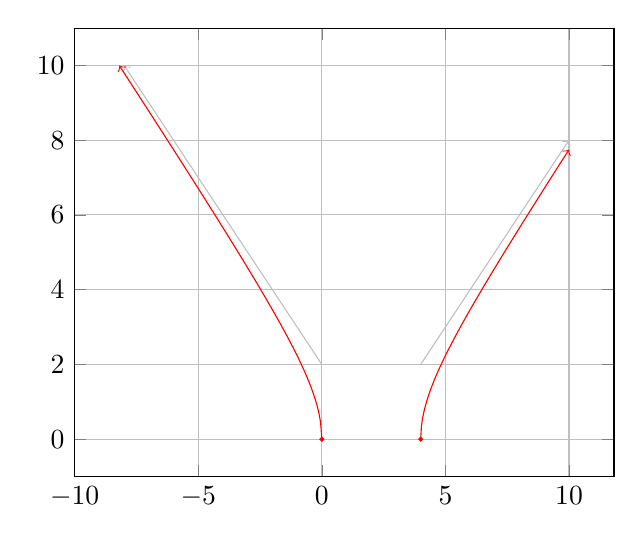
\begin{tikzpicture}
      \begin{axis}[domain=-10:10,
        restrict y to domain=-10:10,
        samples=200,
        grid=both]
        \addplot[lightgray,domain=-10:0,<-] { -x+2 };
        \addplot[lightgray,domain=4:10,->] { x-2 };
        \addplot[red,domain=-10:0,<-] { sqrt(x^2-4*x) };
        \addplot[red,domain=4:10,->] { sqrt(x^2-4*x) };
        \node[draw=red,fill=red,circle,inner sep=0.5pt]
        at (axis cs: 0,0) {};        
        \node[draw=red,fill=red,circle,inner sep=0.5pt]
        at (axis cs: 4,0) {};        
      \end{axis}
    \end{tikzpicture}
    \caption{Graph of $\ds y=\sqrt{x^2-4x}$}
    \label{fig:sqrtx2-4x}
  \end{figure}    
\end{enumerate}
\end{document}


